\subsection{Experiment One}
The 1000 hour graph Figure is shown in \ref{fig:fullPageExperiment1} for the best prediction from Experiment One. The full graph can be seen in the digitalized version. In the directory "PriceGraphExperiment1".

\begin{sidewaysfigure}[h]
\centering
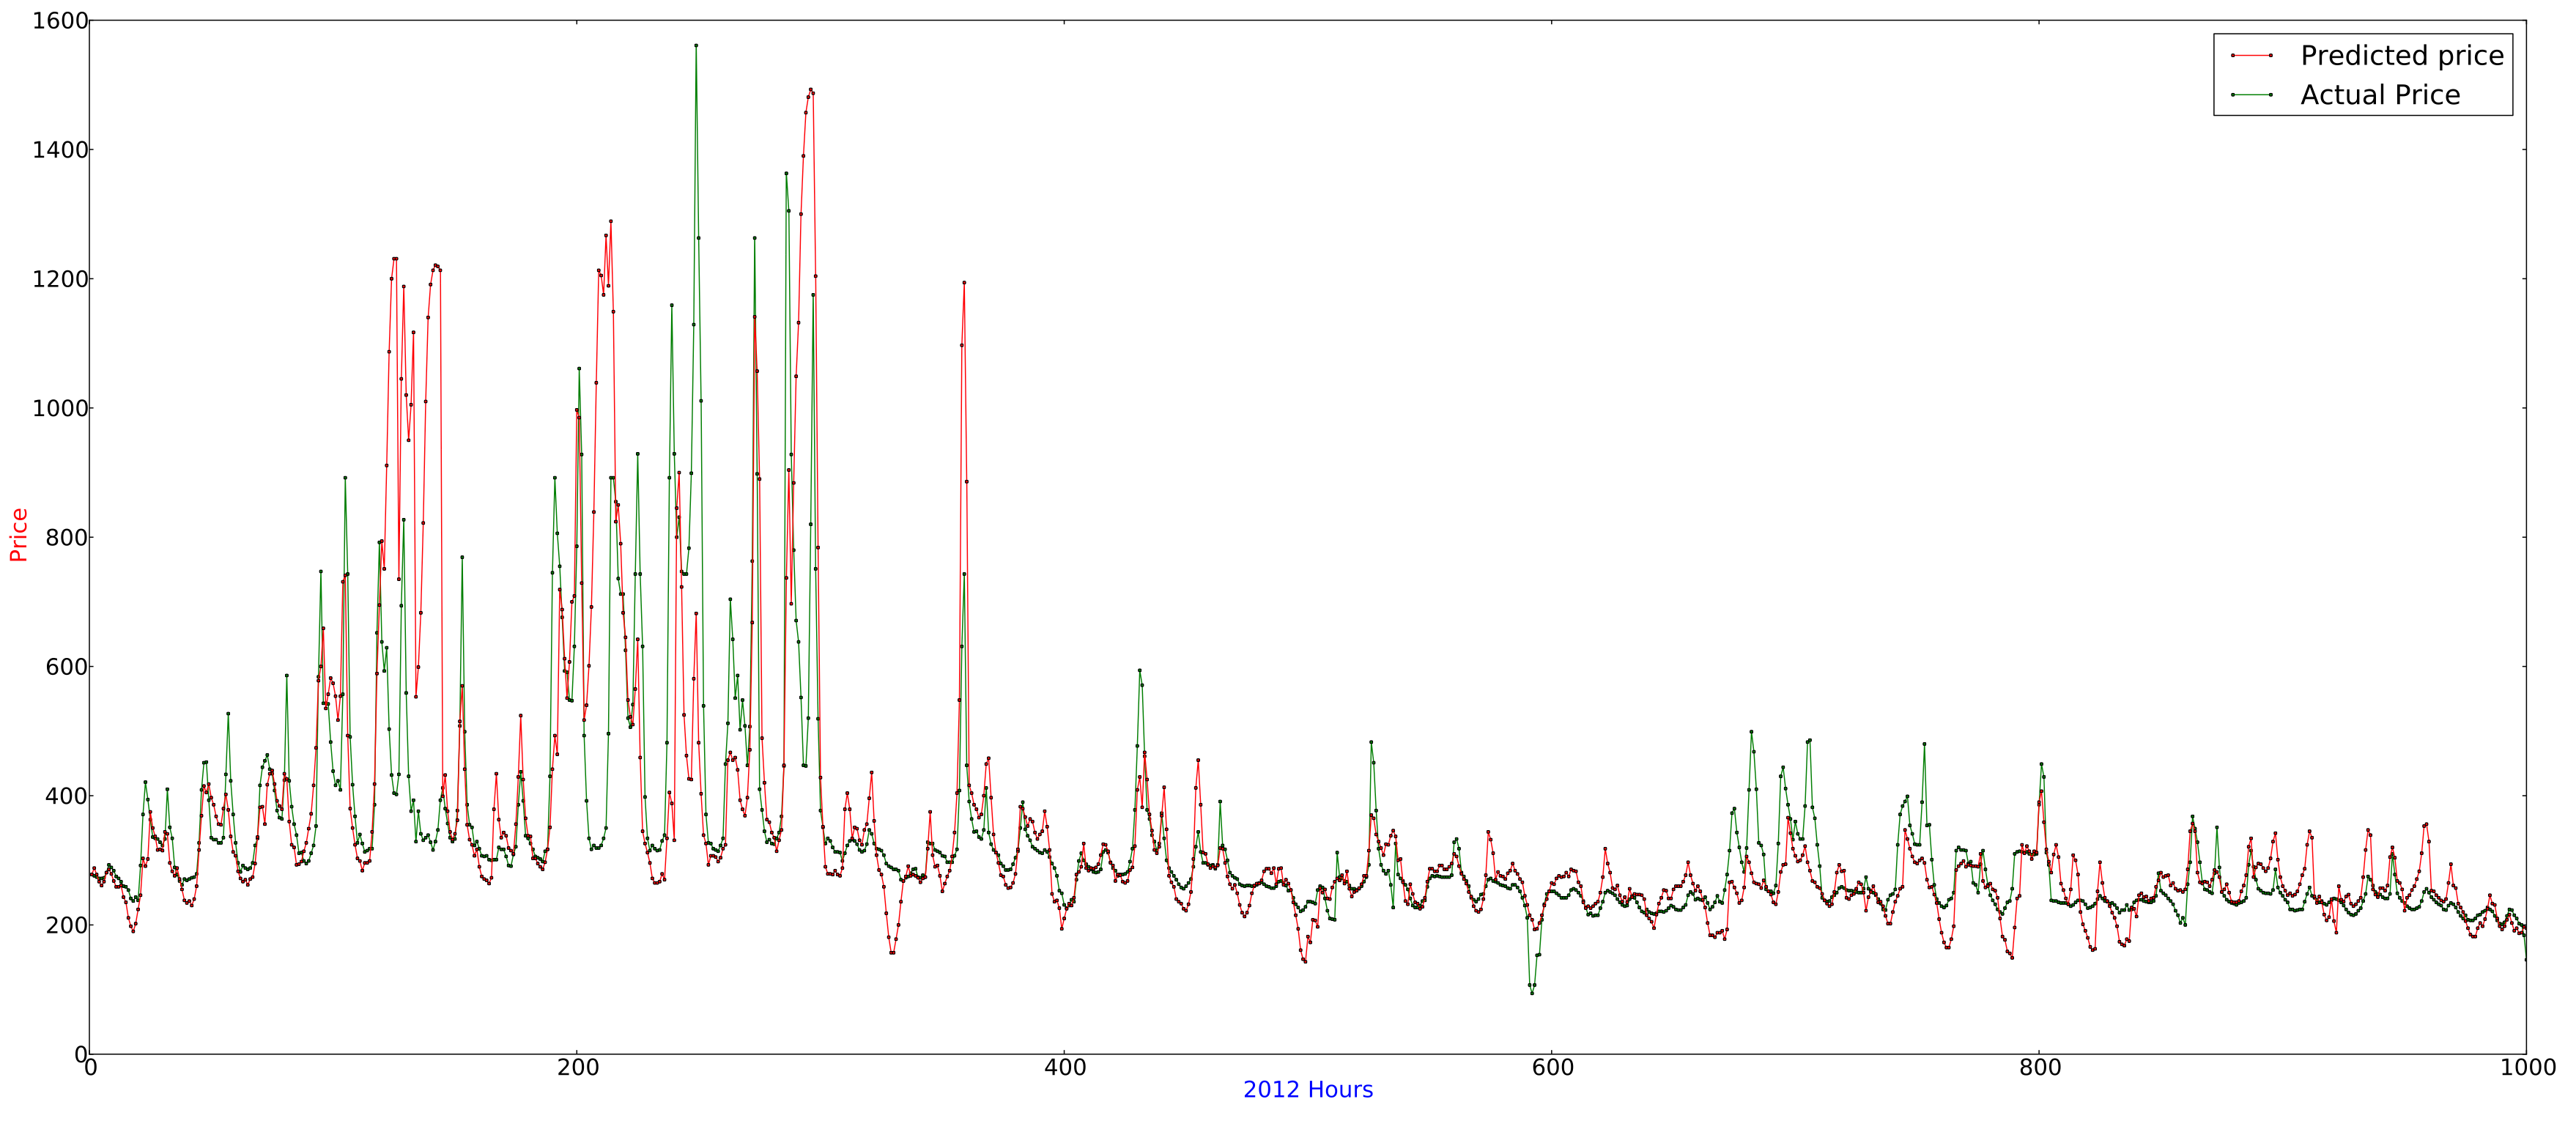
\includegraphics[width=\linewidth]{billeder/PriceGraphs/Experiment1.png}
\caption{First 1000 hours of the best prediction in experiment 1}
\label{fig:fullPageExperiment1}
\end{sidewaysfigure}

This includes last hours Price (P), The Demand (D), Wind Speed(WS), Temperature(T), The Hourly Time of Day (ToD), The Day of The Week(DoW), The Month of The Year(MoY), The Season of The Year(SoY),

\footnotesize
\begin{longtable}{|c|c|c|c|c|c|c|c|c|c|c|c|c|c|}
\caption{Input parameters test}\\
\hline
\textbf{\#} & \textbf{P} & \textbf{C} & \textbf{WS} & \textbf{T} & \textbf{ToD} & \textbf{DoW} & \textbf{MoY}& \textbf{SoY} & \textbf{Trend} & \textbf{H1} & \textbf{H2} & \textbf{MAE} & \textbf{\% Deviation} \\
\hline
\endfirsthead
\multicolumn{10}{c}%
{\tablename\ \thetable\ -- \textit{Continued from previous page}} \\
\hline
\textbf{\#} & \textbf{P} & \textbf{C} & \textbf{WS} & \textbf{T} & \textbf{ToD} & \textbf{DoW} & \textbf{MoY}& \textbf{SoY} & \textbf{Trend} & \textbf{H1} & \textbf{H2} & \textbf{MAE} & \textbf{\% Deviation} \\
\hline
\endhead
\hline \multicolumn{10}{r}{\textit{Continued on next page}} \\
\endfoot
\hline
\endlastfoot
1   &  \x    & \x    & \x    & \x    & \x\m  & \x\m  &       & \x\m  & 66,8\% &  7  & 8  & 57,12 & - \\ \hline
2   &  \x    & \x    & \x    & \x    & \x\m  & \x    &       & \x\m  & 67,9\% &  5  & 9  & 58,09 & 1,7\% \\ \hline
3   &  \x    & \x    & \x    & \x    & \x\m  &       & \x\m  &       & 66,5\% &  6  & 11 & 58,79 & 2,92\% \\ \hline
4   &  \x    & \x    & \x    &       & \x\m  & \x\m  & \x\m  &       & 66,5\% &  9  & 3  & 60,14 & 5,29\% \\ \hline
5   &  \x    & \x    & \x    & \x    & \x\m  & \x    &       &       & 66,9\% &  16 & 8  & 62,19 & 8,88\% \\ \hline
6   &  \x    & \x    & \x    & \x    & \x\m  &       &       & \x\m  & 67,2\% &  6  & 5  & 62,26 & 9,0\% \\ \hline
7   &  \x    & \x    & \x    & \x    & \x\m  & \x    & \x\m  &       & 67,0\% &  5  & 8  & 62,84 & 10,01\% \\ \hline
8   &  \x    & \x    & \x    & \x    & \x    & \x    &       & \x\m  & 62,9\% &  5  & 0  & 63,94 & 11,94\% \\ \hline
9   &  \x    & \x    & \x    & \x    & \x    & \x\m  & \x\m  &       & 62,2\% &  5  & 4  & 64,19 & 12,38\% \\ \hline
10  &  \x    & \x    & \x    &       & \x\m  & \x    & \x\m  &       & 67,4\% &  6  & 8  & 64,72 & 13,31\% \\ \hline
11  &  \x    & \x    & \x    &       & \x    & \x    & \x\m  &       & 63,3\% &  5  & 5  & 65,07 & 13,92\% \\ \hline
12  &  \x    & \x    & \x    & \x    & \x\m  & \x\m  &       &       & 67,0\% &  6  & 6  & 65,95 & 15,46\% \\ \hline
13  &  \x    & \x    & \x    & \x    & \x\m  & \x\m  & \x\m  &       & 66,8\% &  7  & 12 & 66,55 & 16,51\% \\ \hline
14  &  \x    & \x    & \x    &       & \x    &       &       & \x\m  & 62,4\% &  7  & 0  & 67,21 & 17,66\% \\ \hline
15  &  \x    & \x    & \x    & \x    & \x    & \x    &       &       & 62,6\% &  5  & 0  & 67,88 & 18,84\% \\ \hline
16  &  \x    & \x    & \x    &       & \x    & \x    &       & \x    & 62,0\% &  6  & 0  & 68,21 & 19,42\% \\ \hline
17  &  \x    & \x    & \x    &       & \x\m  & \x\m  &       &       & 67,2\% &  8  & 6  & 68,34 & 19,64\% \\ \hline
18  &  \x    & \x    & \x    &       & \x\m  &       &       & \x\m  & 68,2\% &  7  & 4  & 68,35 & 19,66\% \\ \hline
19  &  \x    & \x    & \x    & \x    & \x    & \x    & \x    &       & 62,2\% &  6  & 0  & 68,43 & 19,8\% \\ \hline
20  &  \x    & \x    & \x    & \x    & \x    &       &       & \x\m  & 62,4\% &  5  & 0  & 68,45 & 19,84\% \\ \hline
21  &  \x    & \x    & \x    &       & \x    &       &       &       & 63,0\% &  5  & 0  & 69,09 & 20,96\% \\ \hline
22  &  \x    & \x    & \x    & \x    &       & \x    &       &       & 62,0\% &  5  & 0  & 69,14 & 21,04\% \\ \hline
23  &  \x    & \x    & \x    &       & \x    &       & \x    &       & 62,2\% &  5  & 0  & 69,34 & 21,39\% \\ \hline
24  &  \x    & \x    & \x    & \x    & \x\m  & \x    & \x    &       & 66,7\% &  7  & 8  & 69,37 & 21,45\% \\ \hline
25  &  \x    & \x    & \x    & \x    & \x\m  &       &       & \x\m  & 67,5\% &  9  & 6  & 69,46 & 21,6\% \\ \hline
26  &  \x    & \x    & \x    & \x    & \x    & \x\m  & \x    &       & 61,5\% &  6  & 0  & 69,47 & 21,62\% \\ \hline
27  &  \x    & \x    & \x    & \x    &       & \x\m  &       &       & 60,7\% &  8  & 0  & 69,50 & 21,67\% \\ \hline
28  &  \x    & \x    & \x    & \x    & \x    &       &       &       & 62,5\% &  11 & 0  & 69,62 & 21,88\% \\ \hline
29  &  \x    & \x    & \x    & \x    &       & \x    & \x    &       & 61,4\% &  5  & 0  & 69,70 & 22,02\% \\ \hline
30  &  \x    & \x    & \x    & \x    & \x\m  &       &       & \x    & 66,6\% &  6  & 0  & 69,71 & 22,04\% \\ \hline
31  &  \x    & \x    & \x    &       & \x    &       &       & \x    & 62,1\% &  6  & 0  & 69,75 & 22,11\% \\ \hline
32  &  \x    & \x    & \x    & \x    & \x    &       & \x    &       & 62,7\% &  7  & 0  & 69,82 & 22,23\% \\ \hline
33  &  \x    & \x    & \x    &       &       &       &       &       & 58,9\% &  6  & 0  & 69,90 & 22,37\% \\ \hline
34  &  \x    & \x    & \x    & \x    &       & \x\m  & \x    &       & 61,3\% &  5  & 0  & 70,29 & 23,06\% \\ \hline
35  &  \x    & \x    & \x    &       & \x    & \x    & \x    &       & 63,0\% &  5  & 0  & 70,58 & 23,56\% \\ \hline
36  &  \x    & \x    & \x    & \x    & \x    & \x    &       & \x    & 61,8\% &  6  & 0  & 70,75 & 23,86\% \\ \hline
37  &  \x    & \x    & \x    &       & \x    & \x    &       & \x\m  & 62,4\% &  5  & 0  & 70,96 & 24,23\% \\ \hline
38  &  \x    & \x    & \x    & \x    &       &       &       &       & 61,3\% &  5  & 0  & 71,31 & 24,84\% \\ \hline
39  &  \x    & \x    &       & \x    & \x\m  & \x\m  &       &       & 67,5\% &  9  & 19 & 71,39 & 24,98\% \\ \hline
40  &  \x    & \x    & \x    &       & \x    & \x    &       &       & 62,2\% &  5  & 0  & 71,49 & 25,16\% \\ \hline
41  &  \x    & \x    & \x    & \x    &       &       &       &       & 60,6\% &  9  & 0  & 71,58 & 25,32\% \\ \hline
42  &  \x    & \x    & \x    & \x    &       & \x    &       & \x\m  & 61,5\% &  6  & 0  & 71,74 & 25,6\% \\ \hline
43  &  \x    & \x    & \x    &       & \x\m  &       & \x\m  &       & 66,7\% &  6  & 11 & 71,81 & 25,72\% \\ \hline
44  &  \x    & \x    & \x    &       & \x\m  & \x\m  &       & \x\m  & 66,8\% &  7  & 5  & 71,89 & 25,86\% \\ \hline
45  &  \x    & \x    & \x    & \x    & \x\m  & \x    &       & \x    & 66,4\% &  8  & 7  & 71,92 & 25,91\% \\ \hline
46  &  \x    & \x    & \x    &       & \x\m  &       &       & \x\m  & 67,2\% &  7  & 10 & 72,70 & 27,28\% \\ \hline
47  &  \x    & \x    & \x    &       & \x\m  & \x    &       & \x    & 66,4\% &  5  & 9  & 72,74 & 27,35\% \\ \hline
48  &  \x    & \x    & \x    & \x    & \x\m  &       &       &       & 66,7\% &  7  & 0  & 73,70 & 29,03\% \\ \hline
49  &  \x    & \x    & \x    & \x    &       & \x    & \x\m  &       & 62,1\% &  6  & 0  & 73,80 & 29,2\% \\ \hline
50  &  \x    & \x    & \x    & \x    &       & \x\m  & \x\m  &       & 61,2\% &  8  & 0  & 74,19 & 29,88\% \\ \hline
51  &  \x    & \x    & \x    & \x    & \x    &       & \x\m  &       & 62,9\% &  10 & 0  & 74,29 & 30,06\% \\ \hline
52  &  \x    & \x    & \x    &       & \x\m  & \x    &       &       & 67,5\% &  8  & 0  & 74,56 & 30,53\% \\ \hline
53  &  \x    & \x    & \x    &       & \x    & \x\m  & \x\m  &       & 62,5\% &  5  & 7  & 74,89 & 31,11\% \\ \hline
54  &  \x    & \x    & \x    &       & \x\m  & \x    &       & \x\m  & 68,0\% &  5  & 3  & 75,25 & 31,74\% \\ \hline
55  &  \x    & \x    & \x    & \x    &       & \x\m  &       & \x\m  & 60,7\% &  7  & 0  & 75,31 & 31,85\% \\ \hline
56  &  \x    & \x    & \x    & \x    & \x    & \x    & \x\m  &       & 62,1\% &  7  & 0  & 75,40 & 32,0\% \\ \hline
57  &  \x    & \x    & \x    & \x    & \x    & \x\m  &       &       & 62,5\% &  5  & 0  & 75,45 & 32,09\% \\ \hline
58  &  \x    & \x    & \x    &       &       &       &       & \x\m  & 59,3\% &  12 & 0  & 75,52 & 32,21\% \\ \hline
59  &  \x    & \x    & \x    &       &       & \x    &       &       & 59,2\% &  5  & 0  & 75,63 & 32,41\% \\ \hline
60  &  \x    & \x    & \x    &       & \x\m  &       &       &       & 67,4\% &  5  & 11 & 75,77 & 32,65\% \\ \hline
61  &  \x    & \x    & \x    & \x    &       & \x\m  &       & \x\m  & 61,6\% &  8  & 0  & 76,12 & 33,26\% \\ \hline
62  &  \x    & \x    & \x    & \x    &       &       & \x\m  &       & 62,5\% &  8  & 0  & 76,18 & 33,37\% \\ \hline
63  &  \x    & \x    & \x    & \x    & \x    & \x\m  &       & \x\m  & 62,2\% &  6  & 0  & 76,19 & 33,39\% \\ \hline
64  &  \x    & \x    & \x    &       &       &       &       &       & 59,7\% &  10 & 0  & 76,32 & 33,61\% \\ \hline
65  &  \x    & \x    & \x    &       & \x    &       & \x\m  &       & 63,0\% &  8  & 0  & 76,39 & 33,74\% \\ \hline
66  &  \x    & \x    & \x    & \x    & \x\m  &       & \x\m  &       & 66,3\% &  8  & 7  & 77,70 & 36,03\% \\ \hline
67  &  \x    & \x    & \x    &       & \x\m  & \x    & \x    &       & 66,9\% &  5  & 0  & 77,72 & 36,06\% \\ \hline
68  &  \x    & \x    & \x    & \x    & \x\m  &       & \x    &       & 67,1\% &  5  & 0  & 78,05 & 36,64\% \\ \hline
69  &  \x    & \x    & \x    & \x    &       & \x\m  &       & \x    & 61,1\% &  9  & 0  & 78,49 & 37,41\% \\ \hline
70  &  \x    & \x    &       & \x    & \x\m  & \x\m  &       & \x\m  & 66,9\% &  12 & 10 & 78,57 & 37,55\% \\ \hline
71  &  \x    & \x    & \x    & \x    & \x    &       &       & \x    & 61,8\% &  7  & 0  & 78,69 & 37,76\% \\ \hline
72  &  \x    & \x    & \x    &       & \x    & \x\m  &       & \x\m  & 61,8\% &  6  & 0  & 78,74 & 37,85\% \\ \hline
73  &  \x    & \x    & \x    &       & \x    & \x\m  &       &       & 62,2\% &  7  & 0  & 78,88 & 38,1\% \\ \hline
74  &  \x    & \x    &       & \x    & \x    & \x    &       &       & 58,2\% &  5  & 0  & 79,01 & 38,32\% \\ \hline
75  &  \x    & \x    &       &       & \x\m  & \x\m  & \x\m  &       & 65,8\% &  16 & 6  & 79,71 & 39,55\% \\ \hline
76  &  \x    & \x    & \x    & \x    &       &       & \x    &       & 62,1\% &  6  & 0  & 79,89 & 39,86\% \\ \hline
77  &  \x    & \x    & \x    &       &       & \x\m  &       & \x\m  & 59,3\% &  8  & 0  & 80,20 & 40,41\% \\ \hline
78  &  \x    & \x    & \x    & \x    & \x    & \x\m  &       & \x    & 62,7\% &  5  & 7  & 81,11 & 42,0\% \\ \hline
79  &  \x    & \x    &       &       &       &       &       &       & 53,1\% &  13 & 0  & 81,28 & 42,3\% \\ \hline
80  &  \x    & \x    & \x    & \x    &       & \x    &       & \x    & 61,1\% &  6  & 0  & 81,34 & 42,4\% \\ \hline
81  &  \x    & \x    &       &       & \x\m  & \x\m  &       & \x\m  & 66,4\% &  15 & 9  & 81,58 & 42,82\% \\ \hline
82  &  \x    & \x    & \x    & \x    &       &       &       & \x\m  & 61,2\% &  9  & 0  & 82,03 & 43,61\% \\ \hline
83  &  \x    & \x    & \x    &       & \x    & \x\m  & \x    &       & 62,4\% &  5  & 0  & 82,04 & 43,63\% \\ \hline
84  &  \x    & \x    &       & \x    & \x    &       &       &       & 59,0\% &  11 & 0  & 82,29 & 44,07\% \\ \hline
85  &  \x    & \x    & \x    &       &       & \x\m  &       &       & 58,7\% &  8  & 0  & 82,32 & 44,12\% \\ \hline
86  &  \x    & \x    &       & \x    &       &       &       &       & 53,9\% &  8  & 0  & 82,72 & 44,82\% \\ \hline
87  &  \x    & \x    &       &       & \x    &       &       &       & 59,6\% &  8  & 0  & 83,35 & 45,92\% \\ \hline
88  &  \x    & \x    & \x    &       & \x\m  &       & \x    &       & 66,6\% &  7  & 0  & 83,82 & 46,74\% \\ \hline
89  &  \x    & \x    & \x    &       & \x    & \x\m  &       & \x    & 62,0\% &  6  & 0  & 84,08 & 47,2\% \\ \hline
90  &  \x    & \x    &       & \x    & \x\m  & \x\m  & \x\m  &       & 65,4\% &  9  & 12 & 84,50 & 47,93\% \\ \hline
91  &  \x    & \x    &       &       & \x\m  & \x\m  &       &       & 67,0\% &  11 & 9  & 85,15 & 49,07\% \\ \hline
92  &  \x    & \x    &       & \x    & \x\m  &       &       & \x\m  & 66,5\% &  11 & 12 & 85,51 & 49,7\% \\ \hline
93  &  \x    & \x    & \x    &       &       &       & \x    &       & 60,7\% &  9  & 0  & 85,55 & 49,77\% \\ \hline
94  &  \x    & \x    & \x    &       &       & \x    &       & \x    & 59,4\% &  6  & 0  & 85,57 & 49,81\% \\ \hline
95  &  \x    & \x    & \x    &       &       &       &       & \x    & 59,7\% &  6  & 0  & 85,66 & 49,96\% \\ \hline
96  &  \x    & \x    & \x    &       & \x\m  &       & \x\m  &       & 66,1\% &  10 & 6  & 85,77 & 50,16\% \\ \hline
97  &  \x    & \x    & \x    &       &       & \x    & \x    &       & 59,9\% &  5  & 0  & 85,99 & 50,54\% \\ \hline
98  &  \x    & \x    &       &       & \x    & \x    &       &       & 58,0\% &  5  & 0  & 86,00 & 50,56\% \\ \hline
99  &  \x    & \x    & \x    &       & \x\m  &       &       & \x    & 66,4\% &  7  & 0  & 86,13 & 50,79\% \\ \hline
100 &  \x    & \x    &       & \x    &       & \x    &       &       & 53,5\% &  5  & 0  & 86,33 & 51,14\% \\ \hline
101 &  \x    & \x    &       &       & \x\m  &       &       & \x\m  & 66,9\% &  15 & 4  & 87,00 & 52,31\% \\ \hline
102 &  \x    & \x    & \x    &       &       & \x    &       & \x\m  & 59,0\% &  7  & 0  & 87,63 & 53,41\% \\ \hline
103 &  \x    & \x    & \x    & \x    &       & \x\m  & \x\m  &       & 61,6\% &  7  & 0  & 87,87 & 53,83\% \\ \hline
104 &  \x    & \x    &       &       &       & \x    &       &       & 51,7\% &  5  & 3  & 87,89 & 53,87\% \\ \hline
105 &  \x    & \x    &       & \x    &       &       &       &       & 53,6\% &  6  & 0  & 87,94 & 53,96\% \\ \hline
106 &  \x    & \x    &       &       &       &       &       &       & 52,6\% &  12 & 0  & 89,03 & 55,86\% \\ \hline
107 &  \x    & \x    & \x    &       &       & \x    & \x\m  &       & 60,2\% &  6  & 0  & 89,14 & 56,06\% \\ \hline
108 &  \x    & \x    & \x    & \x    &       &       &       & \x    & 60,9\% &  7  & 0  & 89,55 & 56,78\% \\ \hline
109 &  \x    & \x    &       &       & \x    & \x    & \x    &       & 57,1\% &  6  & 0  & 90,73 & 58,84\% \\ \hline
110 &  \x    & \x    &       & \x    & \x\m  &       &       &       & 65,7\% &  11 & 0  & 91,06 & 59,42\% \\ \hline
111 &  \x    & \x    &       &       & \x\m  &       &       &       & 67,4\% &  11 & 0  & 91,23 & 59,72\% \\ \hline
112 &  \x    & \x    &       &       &       &       &       & \x\m  & 52,6\% &  13 & 0  & 91,67 & 60,49\% \\ \hline
113 &  \x    & \x    & \x    &       &       & \x\m  &       & \x\m  & 59,2\% &  7  & 0  & 91,91 & 60,91\% \\ \hline
114 &  \x    & \x    & \x    &       &       & \x\m  & \x\m  &       & 59,6\% &  6  & 0  & 92,65 & 62,2\% \\ \hline
115 &  \x    & \x    &       & \x    & \x    & \x    &       & \x    & 56,5\% &  5  & 0  & 92,95 & 62,73\% \\ \hline
116 &  \x    & \x    & \x    &       &       &       & \x\m  &       & 60,2\% &  9  & 0  & 93,63 & 63,92\% \\ \hline
117 &  \x    & \x    & \x    &       &       & \x\m  & \x    &       & 59,3\% &  9  & 0  & 94,58 & 65,58\% \\ \hline
118 &  \x    & \x    &       &       &       &       &       & \x    & 52,3\% &  6  & 0  & 96,70 & 69,29\% \\ \hline
119 &  \x    & \x    &       &       &       & \x\m  &       &       & 50,0\% &  7  & 0  & 96,78 & 69,43\% \\ \hline
120 &  \x    & \x    &       &       & \x    &       &       & \x    & 57,2\% &  6  & 0  & 97,09 & 69,98\% \\ \hline
121 &  \x    & \x    &       & \x    & \x    & \x    & \x    &       & 56,7\% &  5  & 0  & 98,17 & 71,87\% \\ \hline
122 &  \x    & \x    &       &       & \x    & \x    &       & \x    & 57,1\% &  6  & 0  & 99,10 & 73,49\% \\ \hline
123 &  \x    & \x    &       &       &       &       & \x    &       & 52,6\% &  8  & 0  & 99,38 & 73,98\% \\ \hline
124 &  \x    & \x    &       &       & \x    &       & \x    &       & 56,8\% &  6  & 0  & 99,78 & 74,68\% \\ \hline
125 &  \x    & \x    & \x    &       &       & \x\m  &       & \x    & 59,0\% &  5  & 0  & 100,63 & 76,17\% \\ \hline
126 &  \x    & \x    &       & \x    &       &       &       & \x\m  & 53,1\% &  8  & 0  & 102,76 & 79,9\% \\ \hline
127 &  \x    & \x    &       & \x    & \x\m  &       & \x\m  &       & 64,9\% &  13 & 16 & 103,01 & 80,34\% \\ \hline
128 &  \x    & \x    &       &       &       & \x    & \x    &       & 51,2\% &  6  & 0  & 103,56 & 81,3\% \\ \hline
129 &  \x    & \x    &       &       &       & \x    &       & \x    & 52,3\% &  5  & 0  & 103,71 & 81,57\% \\ \hline
130 &  \x    & \x    &       & \x    &       & \x    &       & \x    & 52,2\% &  5  & 0  & 104,19 & 82,41\% \\ \hline
131 &  \x    & \x    &       & \x    &       & \x\m  &       &       & 53,0\% &  9  & 0  & 104,33 & 82,65\% \\ \hline
132 &  \x    & \x    &       &       & \x\m  &       & \x\m  &       & 66,0\% &  12 & 14 & 104,93 & 83,7\% \\ \hline
133 &  \x    & \x    &       & \x    & \x    &       &       & \x    & 56,3\% &  5  & 0  & 105,04 & 83,89\% \\ \hline
134 &  \x    & \x    & \x    &       &       & \x\m  & \x\m  &       & 59,8\% &  5  & 0  & 105,70 & 85,05\% \\ \hline
135 &  \x    & \x    &       &       &       & \x\m  &       & \x\m  & 51,4\% &  7  & 0  & 107,85 & 88,81\% \\ \hline
136 &  \x    & \x    &       & \x    & \x    &       & \x    &       & 56,5\% &  5  & 0  & 108,37 & 89,72\% \\ \hline
137 &  \x    & \x    &       & \x    &       &       & \x    &       & 54,4\% &  7  & 0  & 111,14 & 94,57\% \\ \hline
138 &  \x    & \x    &       & \x    &       &       & \x\m  &       & 53,5\% &  8  & 0  & 111,65 & 95,47\% \\ \hline
139 &  \x    & \x    &       & \x    &       & \x\m  & \x\m  &       & 52,9\% &  7  & 0  & 113,56 & 98,81\% \\ \hline
140 &  \x    & \x    &       & \x    &       &       &       & \x    & 52,7\% &  8  & 0  & 115,29 & 101,84\% \\ \hline
141 &  \x    & \x    &       &       &       &       & \x\m  &       & 53,0\% &  11 & 0  & 115,81 & 102,75\% \\ \hline
142 &  \x    & \x    &       & \x    &       & \x\m  &       & \x\m  & 53,0\% &  5  & 0  & 115,83 & 102,78\% \\ \hline
143 &  \x    & \x    &       & \x    &       & \x    & \x    &       & 53,2\% &  6  & 0  & 117,17 & 105,13\% \\ \hline
144 &  \x    & \x    &       &       &       & \x\m  & \x\m  &       & 52,0\% &  7  & 0  & 117,34 & 105,43\% \\ \hline
\end{longtable}
\normalsize

\footnotesize
\begin{longtable}{|c|c|c|c|c|c|c|c|c|c|c|c|c|c|}
\caption{Input parameters test}\\
\hline
\textbf{\#} & \textbf{P} & \textbf{C} & \textbf{WS} & \textbf{T} & \textbf{ToD} & \textbf{DoW} & \textbf{MoY}& \textbf{SoY} & \textbf{Trend} & \textbf{H1} & \textbf{H2} & \textbf{MAE} & \textbf{\% Deviation} \\
\hline
\endfirsthead
\multicolumn{10}{c}%
{\tablename\ \thetable\ -- \textit{Continued from previous page}} \\
\hline
\textbf{\#} & \textbf{P} & \textbf{C} & \textbf{WS} & \textbf{T} & \textbf{ToD} & \textbf{DoW} & \textbf{MoY}& \textbf{SoY} & \textbf{Trend} & \textbf{H1} & \textbf{H2} & \textbf{MAE} & \textbf{\% Deviation} \\
\hline
\endhead
\hline \multicolumn{10}{r}{\textit{Continued on next page}} \\
\endfoot
\hline
\endlastfoot
1  &  \x    & \x    & \x    & \x    & \x\m  & \x\m  &       &       & 66,9\% &  6  & 5  & 58,19 & - \\ \hline
2  &  \x    & \x    & \x    & \x    & \x\m  & \x\m  &       & \x\m  & 66,9\% &  6  & 0  & 61,70 & 6,03\% \\ \hline
3  &  \x    & \x    & \x    & \x    & \x\m  &       &       & \x\m  & 67,7\% &  9  & 0  & 61,86 & 6,31\% \\ \hline
4  &  \x    & \x    & \x    & \x    & \x\m  & \x    & \x\m  &       & 65,8\% &  5  & 0  & 62,62 & 7,61\% \\ \hline
5  &  \x    & \x    & \x    & \x    & \x    &       &       &       & 60,2\% &  5  & 0  & 62,98 & 8,23\% \\ \hline
6  &  \x    & \x    & \x    & \x    & \x\m  &       & \x\m  &       & 66,6\% &  10 & 0  & 63,80 & 9,64\% \\ \hline
7  &  \x    & \x    & \x    &       & \x\m  &       &       & \x\m  & 66,6\% &  6  & 0  & 64,90 & 11,53\% \\ \hline
8  &  \x    & \x    & \x    &       & \x\m  & \x    &       & \x\m  & 66,4\% &  6  & 0  & 65,32 & 12,25\% \\ \hline
9  &  \x    & \x    & \x    & \x    & \x\m  & \x    & \x    &       & 65,9\% &  5  & 0  & 66,42 & 14,14\% \\ \hline
10 &  \x    & \x    & \x    &       & \x    &       &       &       & 61,0\% &  5  & 2  & 66,48 & 14,25\% \\ \hline
11 &  \x    & \x    & \x    &       & \x\m  & \x\m  &       & \x\m  & 66,7\% &  5  & 2  & 67,06 & 15,24\% \\ \hline
12 &  \x    & \x    & \x    & \x    & \x\m  & \x\m  & \x\m  &       & 65,5\% &  7  & 11 & 67,31 & 15,67\% \\ \hline
13 &  \x    & \x    & \x    &       & \x\m  & \x    &       &       & 67,7\% &  6  & 0  & 67,60 & 16,17\% \\ \hline
14 &  \x    & \x    & \x    & \x    & \x\m  &       & \x\m  &       & 65,2\% &  5  & 17 & 67,76 & 16,45\% \\ \hline
15 &  \x    & \x    & \x    &       & \x\m  & \x\m  & \x\m  &       & 65,6\% &  10 & 4  & 67,82 & 16,55\% \\ \hline
16 &  \x    & \x    & \x    &       & \x\m  & \x    & \x    &       & 67,1\% &  5  & 0  & 68,13 & 17,08\% \\ \hline
17 &  \x    & \x    & \x    & \x    & \x\m  & \x    &       & \x\m  & 66,4\% &  5  & 8  & 68,23 & 17,25\% \\ \hline
18 &  \x    & \x    & \x    & \x    & \x\m  &       &       & \x    & 66,4\% &  7  & 6  & 68,41 & 17,56\% \\ \hline
19 &  \x    & \x    & \x    &       & \x    & \x    & \x    &       & 59,7\% &  5  & 0  & 68,43 & 17,6\% \\ \hline
20 &  \x    & \x    &       & \x    & \x\m  & \x\m  &       & \x\m  & 66,2\% &  6  & 0  & 68,63 & 17,94\% \\ \hline
21 &  \x    & \x    & \x    & \x    & \x\m  &       &       & \x\m  & 66,0\% &  5  & 0  & 68,83 & 18,28\% \\ \hline
22 &  \x    & \x    & \x    &       & \x\m  &       & \x    &       & 66,6\% &  6  & 14 & 69,19 & 18,9\% \\ \hline
23 &  \x    & \x    & \x    & \x    & \x\m  & \x    &       & \x    & 67,0\% &  6  & 23 & 69,31 & 19,11\% \\ \hline
24 &  \x    & \x    & \x    &       & \x\m  &       & \x\m  &       & 66,5\% &  6  & 6  & 69,89 & 20,11\% \\ \hline
25 &  \x    & \x    & \x    & \x    & \x    & \x    &       & \x    & 59,0\% &  5  & 0  & 70,28 & 20,78\% \\ \hline
26 &  \x    & \x    & \x    &       & \x\m  &       & \x\m  &       & 66,1\% &  8  & 0  & 70,53 & 21,21\% \\ \hline
27 &  \x    & \x    & \x    & \x    & \x    & \x\m  &       & \x    & 59,5\% &  5  & 0  & 70,60 & 21,33\% \\ \hline
28 &  \x    & \x    & \x    &       & \x    & \x    &       &       & 59,1\% &  5  & 0  & 70,98 & 21,98\% \\ \hline
29 &  \x    & \x    & \x    &       & \x\m  & \x    &       & \x    & 66,0\% &  5  & 0  & 71,30 & 22,53\% \\ \hline
30 &  \x    & \x    & \x    &       & \x    & \x\m  &       &       & 60,2\% &  5  & 3  & 71,44 & 22,77\% \\ \hline
31 &  \x    & \x    & \x    &       &       &       &       &       & 56,6\% &  6  & 0  & 71,96 & 23,66\% \\ \hline
32 &  \x    & \x    & \x    & \x    & \x    &       &       & \x    & 59,6\% &  5  & 0  & 72,02 & 23,77\% \\ \hline
33 &  \x    & \x    & \x    & \x    & \x\m  &       & \x    &       & 66,1\% &  5  & 0  & 72,24 & 24,15\% \\ \hline
34 &  \x    & \x    & \x    &       & \x\m  & \x    & \x\m  &       & 66,3\% &  8  & 0  & 72,29 & 24,23\% \\ \hline
35 &  \x    & \x    & \x    &       & \x\m  & \x\m  &       &       & 66,9\% &  5  & 0  & 72,31 & 24,27\% \\ \hline
36 &  \x    & \x    & \x    & \x    & \x    & \x    &       & \x\m  & 58,8\% &  5  & 0  & 72,37 & 24,37\% \\ \hline
37 &  \x    & \x    & \x    &       & \x    & \x    &       & \x    & 58,7\% &  5  & 0  & 72,45 & 24,51\% \\ \hline
38 &  \x    & \x    & \x    & \x    & \x    & \x\m  &       & \x\m  & 58,9\% &  7  & 0  & 72,91 & 25,3\% \\ \hline
39 &  \x    & \x    &       &       & \x\m  & \x\m  & \x\m  &       & 66,3\% &  8  & 0  & 73,10 & 25,62\% \\ \hline
40 &  \x    & \x    & \x    & \x    & \x\m  &       &       &       & 66,6\% &  8  & 0  & 73,35 & 26,05\% \\ \hline
41 &  \x    & \x    & \x    &       & \x    &       &       & \x    & 58,7\% &  7  & 0  & 73,52 & 26,34\% \\ \hline
42 &  \x    & \x    & \x    &       & \x    & \x\m  &       & \x\m  & 58,9\% &  7  & 0  & 73,57 & 26,43\% \\ \hline
43 &  \x    & \x    & \x    &       &       & \x    &       & \x\m  & 55,4\% &  8  & 0  & 74,26 & 27,62\% \\ \hline
44 &  \x    & \x    &       &       & \x\m  & \x\m  &       &       & 67,1\% &  10 & 0  & 74,48 & 27,99\% \\ \hline
45 &  \x    & \x    & \x    &       & \x    &       &       & \x\m  & 59,9\% &  8  & 0  & 74,67 & 28,32\% \\ \hline
46 &  \x    & \x    & \x    & \x    & \x\m  & \x    &       &       & 67,0\% &  5  & 0  & 74,89 & 28,7\% \\ \hline
47 &  \x    & \x    & \x    &       & \x    &       & \x    &       & 58,6\% &  5  & 0  & 74,96 & 28,82\% \\ \hline
48 &  \x    & \x    & \x    & \x    & \x    & \x    & \x    &       & 59,4\% &  5  & 0  & 75,10 & 29,06\% \\ \hline
49 &  \x    & \x    &       & \x    & \x    &       &       & \x    & 56,4\% &  5  & 0  & 75,31 & 29,42\% \\ \hline
50 &  \x    & \x    & \x    & \x    & \x    & \x    & \x\m  &       & 59,7\% &  5  & 0  & 75,70 & 30,09\% \\ \hline
51 &  \x    & \x    & \x    & \x    & \x    &       &       & \x\m  & 59,3\% &  5  & 4  & 75,97 & 30,56\% \\ \hline
52 &  \x    & \x    &       & \x    & \x\m  &       & \x\m  &       & 65,9\% &  6  & 0  & 76,08 & 30,74\% \\ \hline
53 &  \x    & \x    &       & \x    & \x\m  & \x\m  & \x\m  &       & 65,6\% &  7  & 0  & 76,22 & 30,98\% \\ \hline
54 &  \x    & \x    & \x    &       & \x    & \x\m  & \x    &       & 58,9\% &  7  & 4  & 76,24 & 31,02\% \\ \hline
55 &  \x    & \x    & \x    &       & \x\m  &       &       & \x\m  & 66,2\% &  8  & 0  & 76,25 & 31,04\% \\ \hline
56 &  \x    & \x    &       &       & \x\m  &       &       & \x\m  & 67,2\% &  6  & 9  & 76,30 & 31,12\% \\ \hline
57 &  \x    & \x    &       &       & \x\m  & \x\m  &       & \x\m  & 66,9\% &  8  & 0  & 76,70 & 31,81\% \\ \hline
58 &  \x    & \x    & \x    & \x    &       &       &       &       & 58,8\% &  8  & 0  & 76,74 & 31,88\% \\ \hline
59 &  \x    & \x    &       &       & \x\m  &       &       &       & 67,5\% &  5  & 23 & 76,79 & 31,96\% \\ \hline
60 &  \x    & \x    &       & \x    & \x\m  & \x\m  &       &       & 65,8\% &  5  & 0  & 76,85 & 32,07\% \\ \hline
61 &  \x    & \x    &       & \x    & \x\m  &       &       & \x\m  & 67,2\% &  5  & 0  & 77,05 & 32,41\% \\ \hline
62 &  \x    & \x    & \x    & \x    &       & \x    & \x    &       & 57,5\% &  5  & 0  & 77,20 & 32,67\% \\ \hline
63 &  \x    & \x    & \x    & \x    & \x    & \x    &       &       & 59,3\% &  5  & 0  & 77,29 & 32,82\% \\ \hline
64 &  \x    & \x    & \x    &       &       & \x\m  & \x    &       & 57,1\% &  5  & 0  & 77,32 & 32,88\% \\ \hline
65 &  \x    & \x    & \x    &       & \x    & \x    &       & \x\m  & 59,3\% &  5  & 0  & 77,46 & 33,12\% \\ \hline
66 &  \x    & \x    & \x    & \x    &       &       &       &       & 57,3\% &  8  & 0  & 77,66 & 33,46\% \\ \hline
67 &  \x    & \x    &       &       & \x    &       &       &       & 59,7\% &  9  & 7  & 77,69 & 33,51\% \\ \hline
68 &  \x    & \x    & \x    &       & \x    & \x\m  & \x\m  &       & 60,0\% &  5  & 0  & 77,73 & 33,58\% \\ \hline
69 &  \x    & \x    &       & \x    & \x\m  &       &       &       & 67,1\% &  7  & 0  & 77,79 & 33,68\% \\ \hline
70 &  \x    & \x    & \x    & \x    & \x    & \x\m  & \x    &       & 59,0\% &  5  & 0  & 77,85 & 33,79\% \\ \hline
71 &  \x    & \x    & \x    & \x    &       & \x    &       &       & 56,8\% &  6  & 0  & 78,04 & 34,11\% \\ \hline
72 &  \x    & \x    &       &       & \x\m  &       & \x\m  &       & 65,9\% &  10 & 0  & 78,13 & 34,27\% \\ \hline
73 &  \x    & \x    & \x    &       & \x    & \x\m  &       & \x    & 59,3\% &  5  & 0  & 78,18 & 34,35\% \\ \hline
74 &  \x    & \x    & \x    & \x    &       & \x\m  & \x\m  &       & 58,8\% &  5  & 0  & 78,33 & 34,61\% \\ \hline
75 &  \x    & \x    & \x    & \x    &       &       &       & \x\m  & 57,0\% &  7  & 0  & 79,14 & 36,0\% \\ \hline
76 &  \x    & \x    & \x    &       &       &       &       &       & 55,6\% &  6  & 0  & 79,29 & 36,26\% \\ \hline
77 &  \x    & \x    & \x    &       &       & \x\m  &       & \x\m  & 55,8\% &  6  & 3  & 79,48 & 36,59\% \\ \hline
78 &  \x    & \x    & \x    & \x    &       & \x\m  &       & \x\m  & 57,5\% &  5  & 9  & 79,55 & 36,71\% \\ \hline
79 &  \x    & \x    & \x    &       &       &       &       & \x\m  & 56,6\% &  8  & 0  & 79,64 & 36,86\% \\ \hline
80 &  \x    & \x    &       &       & \x    & \x    &       &       & 58,2\% &  5  & 0  & 79,66 & 36,9\% \\ \hline
81 &  \x    & \x    & \x    &       & \x    & \x    & \x\m  &       & 59,2\% &  6  & 0  & 79,71 & 36,98\% \\ \hline
82 &  \x    & \x    & \x    & \x    &       &       & \x    &       & 57,4\% &  6  & 0  & 80,26 & 37,93\% \\ \hline
83 &  \x    & \x    & \x    &       &       &       & \x    &       & 56,7\% &  5  & 1  & 80,36 & 38,1\% \\ \hline
84 &  \x    & \x    & \x    &       & \x\m  &       &       & \x    & 66,4\% &  5  & 1  & 80,56 & 38,44\% \\ \hline
85 &  \x    & \x    & \x    & \x    &       &       &       & \x    & 58,1\% &  8  & 0  & 81,11 & 39,39\% \\ \hline
86 &  \x    & \x    & \x    &       &       & \x    & \x    &       & 56,0\% &  7  & 0  & 81,45 & 39,97\% \\ \hline
87 &  \x    & \x    & \x    &       &       & \x\m  &       & \x\m  & 55,4\% &  6  & 0  & 81,97 & 40,87\% \\ \hline
88 &  \x    & \x    & \x    & \x    &       & \x\m  &       & \x\m  & 57,1\% &  9  & 0  & 81,98 & 40,88\% \\ \hline
89 &  \x    & \x    & \x    &       & \x\m  &       &       &       & 67,2\% &  9  & 0  & 82,05 & 41,0\% \\ \hline
90 &  \x    & \x    &       &       &       &       &       &       & 51,5\% &  6  & 0  & 82,21 & 41,28\% \\ \hline
91 &  \x    & \x    & \x    & \x    &       & \x    &       & \x    & 57,5\% &  5  & 0  & 82,66 & 42,05\% \\ \hline
92 &  \x    & \x    &       & \x    & \x    & \x    &       &       & 56,9\% &  8  & 0  & 82,70 & 42,12\% \\ \hline
93 &  \x    & \x    & \x    & \x    &       & \x\m  & \x\m  &       & 57,9\% &  7  & 0  & 82,85 & 42,38\% \\ \hline
94 &  \x    & \x    &       &       & \x    & \x    &       & \x    & 55,7\% &  5  & 0  & 82,88 & 42,43\% \\ \hline
95 &  \x    & \x    &       &       & \x    &       &       & \x    & 57,7\% &  5  & 0  & 83,00 & 42,64\% \\ \hline
96 &  \x    & \x    & \x    &       &       & \x    & \x\m  &       & 57,6\% &  6  & 0  & 83,59 & 43,65\% \\ \hline
97 &  \x    & \x    & \x    & \x    & \x    &       & \x\m  &       & 59,1\% &  5  & 0  & 83,76 & 43,94\% \\ \hline
98 &  \x    & \x    &       &       & \x    & \x    & \x    &       & 57,4\% &  10 & 1  & 83,97 & 44,3\% \\ \hline
99 &  \x    & \x    &       & \x    &       & \x    &       &       & 52,4\% &  11 & 0  & 83,98 & 44,32\% \\ \hline
100 &  \x    & \x    & \x    &       &       &       & \x\m  &       & 56,9\% &  10 & 0  & 83,99 & 44,34\% \\ \hline
101 &  \x    & \x    & \x    & \x    & \x    & \x\m  & \x\m  &       & 59,2\% &  8  & 0  & 84,12 & 44,56\% \\ \hline
102 &  \x    & \x    & \x    &       &       & \x    &       & \x    & 55,1\% &  9  & 0  & 84,22 & 44,73\% \\ \hline
103 &  \x    & \x    & \x    & \x    &       & \x    &       & \x\m  & 56,2\% &  8  & 0  & 84,23 & 44,75\% \\ \hline
104 &  \x    & \x    & \x    &       &       & \x    &       &       & 54,2\% &  7  & 0  & 84,31 & 44,89\% \\ \hline
105 &  \x    & \x    & \x    & \x    &       & \x\m  & \x    &       & 57,1\% &  10 & 0  & 85,00 & 46,07\% \\ \hline
106 &  \x    & \x    &       & \x    & \x    &       &       &       & 58,2\% &  12 & 0  & 85,11 & 46,26\% \\ \hline
107 &  \x    & \x    & \x    & \x    &       & \x\m  &       &       & 57,1\% &  8  & 0  & 85,13 & 46,3\% \\ \hline
108 &  \x    & \x    & \x    & \x    &       & \x    & \x\m  &       & 58,5\% &  7  & 0  & 85,22 & 46,45\% \\ \hline
109 &  \x    & \x    &       & \x    & \x    &       & \x    &       & 57,6\% &  5  & 0  & 85,30 & 46,59\% \\ \hline
110 &  \x    & \x    & \x    &       &       & \x\m  & \x\m  &       & 56,8\% &  6  & 9  & 85,35 & 46,67\% \\ \hline
111 &  \x    & \x    & \x    &       &       & \x\m  &       & \x    & 55,9\% &  7  & 0  & 85,99 & 47,77\% \\ \hline
112 &  \x    & \x    &       &       &       & \x\m  &       & \x\m  & 50,2\% &  7  & 0  & 86,42 & 48,51\% \\ \hline
113 &  \x    & \x    & \x    &       &       &       &       & \x    & 56,0\% &  7  & 0  & 86,64 & 48,89\% \\ \hline
114 &  \x    & \x    & \x    & \x    &       &       & \x\m  &       & 58,5\% &  7  & 0  & 87,26 & 49,96\% \\ \hline
115 &  \x    & \x    &       &       &       &       & \x    &       & 51,8\% &  7  & 0  & 87,88 & 51,02\% \\ \hline
116 &  \x    & \x    &       & \x    & \x    & \x    & \x    &       & 56,9\% &  6  & 0  & 88,25 & 51,66\% \\ \hline
117 &  \x    & \x    & \x    &       &       &       &       &       & 55,5\% &  5  & 0  & 89,02 & 52,98\% \\ \hline
118 &  \x    & \x    &       &       &       & \x    & \x    &       & 52,0\% &  6  & 0  & 89,42 & 53,67\% \\ \hline
119 &  \x    & \x    & \x    & \x    &       & \x\m  &       & \x    & 56,5\% &  7  & 0  & 89,94 & 54,56\% \\ \hline
120 &  \x    & \x    &       &       & \x    &       & \x    &       & 55,8\% &  6  & 14 & 90,09 & 54,82\% \\ \hline
121 &  \x    & \x    & \x    &       &       & \x\m  & \x\m  &       & 56,7\% &  5  & 0  & 90,12 & 54,87\% \\ \hline
122 &  \x    & \x    &       & \x    &       &       &       &       & 53,3\% &  8  & 9  & 90,95 & 56,3\% \\ \hline
123 &  \x    & \x    &       &       &       &       &       & \x\m  & 51,8\% &  9  & 0  & 91,05 & 56,47\% \\ \hline
124 &  \x    & \x    &       & \x    &       & \x\m  &       &       & 52,0\% &  6  & 9  & 91,30 & 56,9\% \\ \hline
125 &  \x    & \x    &       & \x    & \x    & \x    &       & \x    & 56,1\% &  6  & 0  & 91,32 & 56,93\% \\ \hline
126 &  \x    & \x    &       & \x    &       &       &       & \x    & 52,0\% &  7  & 0  & 91,69 & 57,57\% \\ \hline
127 &  \x    & \x    & \x    &       &       & \x\m  &       &       & 53,9\% &  8  & 3  & 92,73 & 59,36\% \\ \hline
128 &  \x    & \x    &       & \x    &       &       & \x    &       & 52,4\% &  7  & 4  & 92,82 & 59,51\% \\ \hline
129 &  \x    & \x    &       & \x    &       & \x    & \x    &       & 51,7\% &  6  & 5  & 93,37 & 60,46\% \\ \hline
130 &  \x    & \x    &       & \x    &       &       & \x\m  &       & 53,3\% &  6  & 0  & 93,56 & 60,78\% \\ \hline
131 &  \x    & \x    &       & \x    &       & \x    &       & \x    & 52,2\% &  5  & 0  & 93,59 & 60,84\% \\ \hline
132 &  \x    & \x    &       & \x    &       &       &       &       & 52,9\% &  9  & 0  & 93,69 & 61,01\% \\ \hline
133 &  \x    & \x    &       &       &       &       &       & \x    & 51,6\% &  9  & 0  & 94,34 & 62,12\% \\ \hline
134 &  \x    & \x    &       &       &       &       &       &       & 51,2\% &  15 & 0  & 94,99 & 63,24\% \\ \hline
135 &  \x    & \x    &       & \x    &       &       &       & \x\m  & 53,1\% &  10 & 0  & 96,45 & 65,75\% \\ \hline
136 &  \x    & \x    &       &       &       & \x\m  &       &       & 50,8\% &  9  & 0  & 96,79 & 66,33\% \\ \hline
137 &  \x    & \x    &       &       &       &       & \x\m  &       & 52,1\% &  11 & 0  & 96,94 & 66,59\% \\ \hline
138 &  \x    & \x    &       &       &       & \x    &       &       & 50,0\% &  5  & 0  & 97,94 & 68,31\% \\ \hline
139 &  \x    & \x    &       & \x    &       & \x\m  &       & \x\m  & 51,0\% &  5  & 10 & 100,13 & 72,07\% \\ \hline
140 &  \x    & \x    &       & \x    &       & \x\m  & \x\m  &       & 52,5\% &  5  & 0  & 100,61 & 72,9\% \\ \hline
141 &  \x    & \x    &       &       &       & \x\m  & \x\m  &       & 51,0\% &  9  & 0  & 102,47 & 76,1\% \\ \hline
142 &  \x    & \x    &       &       &       & \x    &       & \x    & 50,9\% &  5  & 0  & 104,56 & 79,69\% \\ \hline
\end{longtable}
\normalsize

\footnotesize
\begin{longtable}{|c|c|c|c|}
\caption{Own set vs Unseen set, Including MAPE}\\
\hline
\textbf{\#} & \textbf{MAE(Training dataset)} & \textbf{MAE(Unseen dataset)} & \textbf{MAPE(Unseen dataset)} \\
\hline
\endfirsthead
\multicolumn{4}{c}%
{\tablename\ \thetable\ -- \textit{Continued from previous page}} \\
\hline
\textbf{\#} & \textbf{MAE(Training dataset)} & \textbf{MAE(Unseen dataset)} & \textbf{MAPE(Unseen dataset)} \\
\hline
\endhead
\hline \multicolumn{4}{r}{\textit{Continued on next page}} \\
\endfoot
\hline
\endlastfoot
	1  & 20,9 & 57,12 & 21,72\% \\ \hline
	2  & 29,61 & 58,09 & 22,09\% \\ \hline
	3  & 25,49 & 58,79 & 22,35\% \\ \hline
	4  & 18,94 & 60,14 & 22,87\% \\ \hline
	5  & 31,1 & 62,19 & 23,65\% \\ \hline
	6  & 22,97 & 62,26 & 23,67\% \\ \hline
	7  & 20,64 & 62,84 & 23,89\% \\ \hline
	8  & 23,87 & 63,94 & 24,31\% \\ \hline
	9  & 17,76 & 64,19 & 24,41\% \\ \hline
	10 & 19,79 & 64,72 & 24,61\% \\ \hline
	11 & 20,85 & 65,07 & 24,74\% \\ \hline
	12 & 25,71 & 65,95 & 25,08\% \\ \hline
	13 & 30,02 & 66,55 & 25,3\% \\ \hline
	14 & 31,32 & 67,21 & 25,56\% \\ \hline
	15 & 31,8 & 67,88 & 25,81\% \\ \hline
	16 & 23,11 & 68,21 & 25,94\% \\ \hline
	17 & 30,39 & 68,34 & 25,98\% \\ \hline
	18 & 40,54 & 68,35 & 25,99\% \\ \hline
	19 & 29,4 & 68,43 & 26,02\% \\ \hline
	20 & 34,38 & 68,45 & 26,03\% \\ \hline
	21 & 43,0 & 69,09 & 26,27\% \\ \hline
	22 & 32,98 & 69,14 & 26,29\% \\ \hline
	23 & 34,93 & 69,34 & 26,36\% \\ \hline
	24 & 79,23 & 69,37 & 26,38\% \\ \hline
	25 & 23,4 & 69,46 & 26,41\% \\ \hline
	26 & 36,0 & 69,47 & 26,41\% \\ \hline
	27 & 40,8 & 69,50 & 26,42\% \\ \hline
	28 & 33,68 & 69,62 & 26,47\% \\ \hline
	29 & 22,59 & 69,70 & 26,5\% \\ \hline
	30 & 22,06 & 69,71 & 26,51\% \\ \hline
	31 & 34,26 & 69,75 & 26,52\% \\ \hline
	32 & 26,2 & 69,82 & 26,55\% \\ \hline
	33 & 45,9 & 69,90 & 26,58\% \\ \hline
	34 & 31,96 & 70,29 & 26,73\% \\ \hline
	35 & 27,24 & 70,58 & 26,84\% \\ \hline
	36 & 22,86 & 70,75 & 26,9\% \\ \hline
	37 & 27,66 & 70,96 & 26,98\% \\ \hline
	38 & 32,6 & 71,31 & 27,11\% \\ \hline
	39 & 43,63 & 71,39 & 27,15\% \\ \hline
	40 & 35,22 & 71,49 & 27,18\% \\ \hline
	41 & 40,97 & 71,58 & 27,22\% \\ \hline
	42 & 26,29 & 71,74 & 27,28\% \\ \hline
	43 & 22,29 & 71,81 & 27,31\% \\ \hline
	44 & 27,08 & 71,89 & 27,33\% \\ \hline
	45 & 27,16 & 71,92 & 27,35\% \\ \hline
	46 & 26,23 & 72,70 & 27,64\% \\ \hline
	47 & 21,52 & 72,74 & 27,66\% \\ \hline
	48 & 28,94 & 73,70 & 28,02\% \\ \hline
	49 & 30,41 & 73,80 & 28,06\% \\ \hline
	50 & 31,81 & 74,19 & 28,21\% \\ \hline
	51 & 22,83 & 74,29 & 28,25\% \\ \hline
	52 & 30,33 & 74,56 & 28,35\% \\ \hline
	53 & 18,98 & 74,89 & 28,48\% \\ \hline
	54 & 47,92 & 75,25 & 28,61\% \\ \hline
	55 & 20,64 & 75,31 & 28,63\% \\ \hline
	56 & 22,16 & 75,40 & 28,67\% \\ \hline
	57 & 33,23 & 75,45 & 28,69\% \\ \hline
	58 & 33,07 & 75,52 & 28,71\% \\ \hline
	59 & 55,33 & 75,63 & 28,76\% \\ \hline
	60 & 29,14 & 75,77 & 28,81\% \\ \hline
	61 & 21,59 & 76,12 & 28,94\% \\ \hline
	62 & 23,15 & 76,18 & 28,97\% \\ \hline
	63 & 23,25 & 76,19 & 28,97\% \\ \hline
	64 & 54,54 & 76,32 & 29,02\% \\ \hline
	65 & 21,57 & 76,39 & 29,05\% \\ \hline
	66 & 21,36 & 77,70 & 29,54\% \\ \hline
	67 & 29,17 & 77,72 & 29,55\% \\ \hline
	68 & 23,47 & 78,05 & 29,68\% \\ \hline
	69 & 25,74 & 78,49 & 29,85\% \\ \hline
	70 & 25,37 & 78,57 & 29,87\% \\ \hline
	71 & 28,61 & 78,69 & 29,92\% \\ \hline
	72 & 23,02 & 78,74 & 29,94\% \\ \hline
	73 & 48,13 & 78,88 & 29,99\% \\ \hline
	74 & 43,03 & 79,01 & 30,04\% \\ \hline
	75 & 38,71 & 79,71 & 30,31\% \\ \hline
	76 & 26,58 & 79,89 & 30,38\% \\ \hline
	77 & 25,86 & 80,20 & 30,5\% \\ \hline
	78 & 19,39 & 81,11 & 30,84\% \\ \hline
	79 & 40,53 & 81,28 & 30,91\% \\ \hline
	80 & 22,61 & 81,34 & 30,93\% \\ \hline
	81 & 27,88 & 81,58 & 31,02\% \\ \hline
	82 & 28,72 & 82,03 & 31,19\% \\ \hline
	83 & 28,02 & 82,04 & 31,19\% \\ \hline
	84 & 35,39 & 82,29 & 31,29\% \\ \hline
	85 & 34,14 & 82,32 & 31,3\% \\ \hline
	86 & 42,64 & 82,72 & 31,45\% \\ \hline
	87 & 70,52 & 83,35 & 31,69\% \\ \hline
	88 & 32,93 & 83,82 & 31,87\% \\ \hline
	89 & 29,08 & 84,08 & 31,97\% \\ \hline
	90 & 42,86 & 84,50 & 32,13\% \\ \hline
	91 & 37,84 & 85,15 & 32,38\% \\ \hline
	92 & 27,01 & 85,51 & 32,51\% \\ \hline
	93 & 29,8 & 85,55 & 32,53\% \\ \hline
	94 & 34,82 & 85,57 & 32,54\% \\ \hline
	95 & 33,33 & 85,66 & 32,57\% \\ \hline
	96 & 38,43 & 85,77 & 32,61\% \\ \hline
	97 & 33,74 & 85,99 & 32,7\% \\ \hline
	98 & 28,01 & 86,00 & 32,7\% \\ \hline
	99 & 27,74 & 86,13 & 32,75\% \\ \hline
	100 & 72,29 & 86,33 & 32,83\% \\ \hline
	101 & 42,09 & 87,00 & 33,08\% \\ \hline
	102 & 41,73 & 87,63 & 33,32\% \\ \hline
	103 & 20,61 & 87,87 & 33,41\% \\ \hline
	104 & 89,21 & 87,89 & 33,42\% \\ \hline
	105 & 46,33 & 87,94 & 33,44\% \\ \hline
	106 & 46,68 & 89,03 & 33,85\% \\ \hline
	107 & 21,15 & 89,14 & 33,89\% \\ \hline
	108 & 26,33 & 89,55 & 34,05\% \\ \hline
	109 & 50,28 & 90,73 & 34,5\% \\ \hline
	110 & 29,26 & 91,06 & 34,62\% \\ \hline
	111 & 50,6 & 91,23 & 34,69\% \\ \hline
	112 & 35,34 & 91,67 & 34,85\% \\ \hline
	113 & 26,64 & 91,91 & 34,95\% \\ \hline
	114 & 20,56 & 92,65 & 35,23\% \\ \hline
	115 & 30,36 & 92,95 & 35,34\% \\ \hline
	116 & 24,38 & 93,63 & 35,6\% \\ \hline
	117 & 25,54 & 94,58 & 35,96\% \\ \hline
	118 & 55,71 & 96,70 & 36,77\% \\ \hline
	119 & 50,05 & 96,78 & 36,8\% \\ \hline
	120 & 31,17 & 97,09 & 36,92\% \\ \hline
	121 & 145,57 & 98,17 & 37,33\% \\ \hline
	122 & 31,64 & 99,10 & 37,68\% \\ \hline
	123 & 76,82 & 99,38 & 37,79\% \\ \hline
	124 & 42,84 & 99,78 & 37,94\% \\ \hline
	125 & 28,13 & 100,63 & 38,26\% \\ \hline
	126 & 36,09 & 102,76 & 39,07\% \\ \hline
	127 & 27,48 & 103,01 & 39,17\% \\ \hline
	128 & 103,76 & 103,56 & 39,38\% \\ \hline
	129 & 43,66 & 103,71 & 39,44\% \\ \hline
	130 & 35,31 & 104,19 & 39,62\% \\ \hline
	131 & 44,97 & 104,33 & 39,67\% \\ \hline
	132 & 32,04 & 104,93 & 39,9\% \\ \hline
	133 & 41,23 & 105,04 & 39,94\% \\ \hline
	134 & 22,81 & 105,70 & 40,19\% \\ \hline
	135 & 42,85 & 107,85 & 41,01\% \\ \hline
	136 & 73,87 & 108,37 & 41,21\% \\ \hline
	137 & 65,42 & 111,14 & 42,26\% \\ \hline
	138 & 43,75 & 111,65 & 42,45\% \\ \hline
	139 & 37,56 & 113,56 & 43,18\% \\ \hline
	140 & 44,47 & 115,29 & 43,84\% \\ \hline
	141 & 38,98 & 115,81 & 44,03\% \\ \hline
	142 & 49,19 & 115,83 & 44,04\% \\ \hline
	143 & 45,62 & 117,17 & 44,55\% \\ \hline
	144 & 39,28 & 117,34 & 44,62\% \\ \hline
	\end{longtable}
\normalsize

\subsection{Experiment Two}
The 1000 hour graph Figure is shown in \ref{fig:fullPageExperiment2} for the best prediction from Experiment Two. The full graph can be seen in the digitalized version. In the directory "PriceGraphExperiment2".

\begin{sidewaysfigure}[h]
\centering
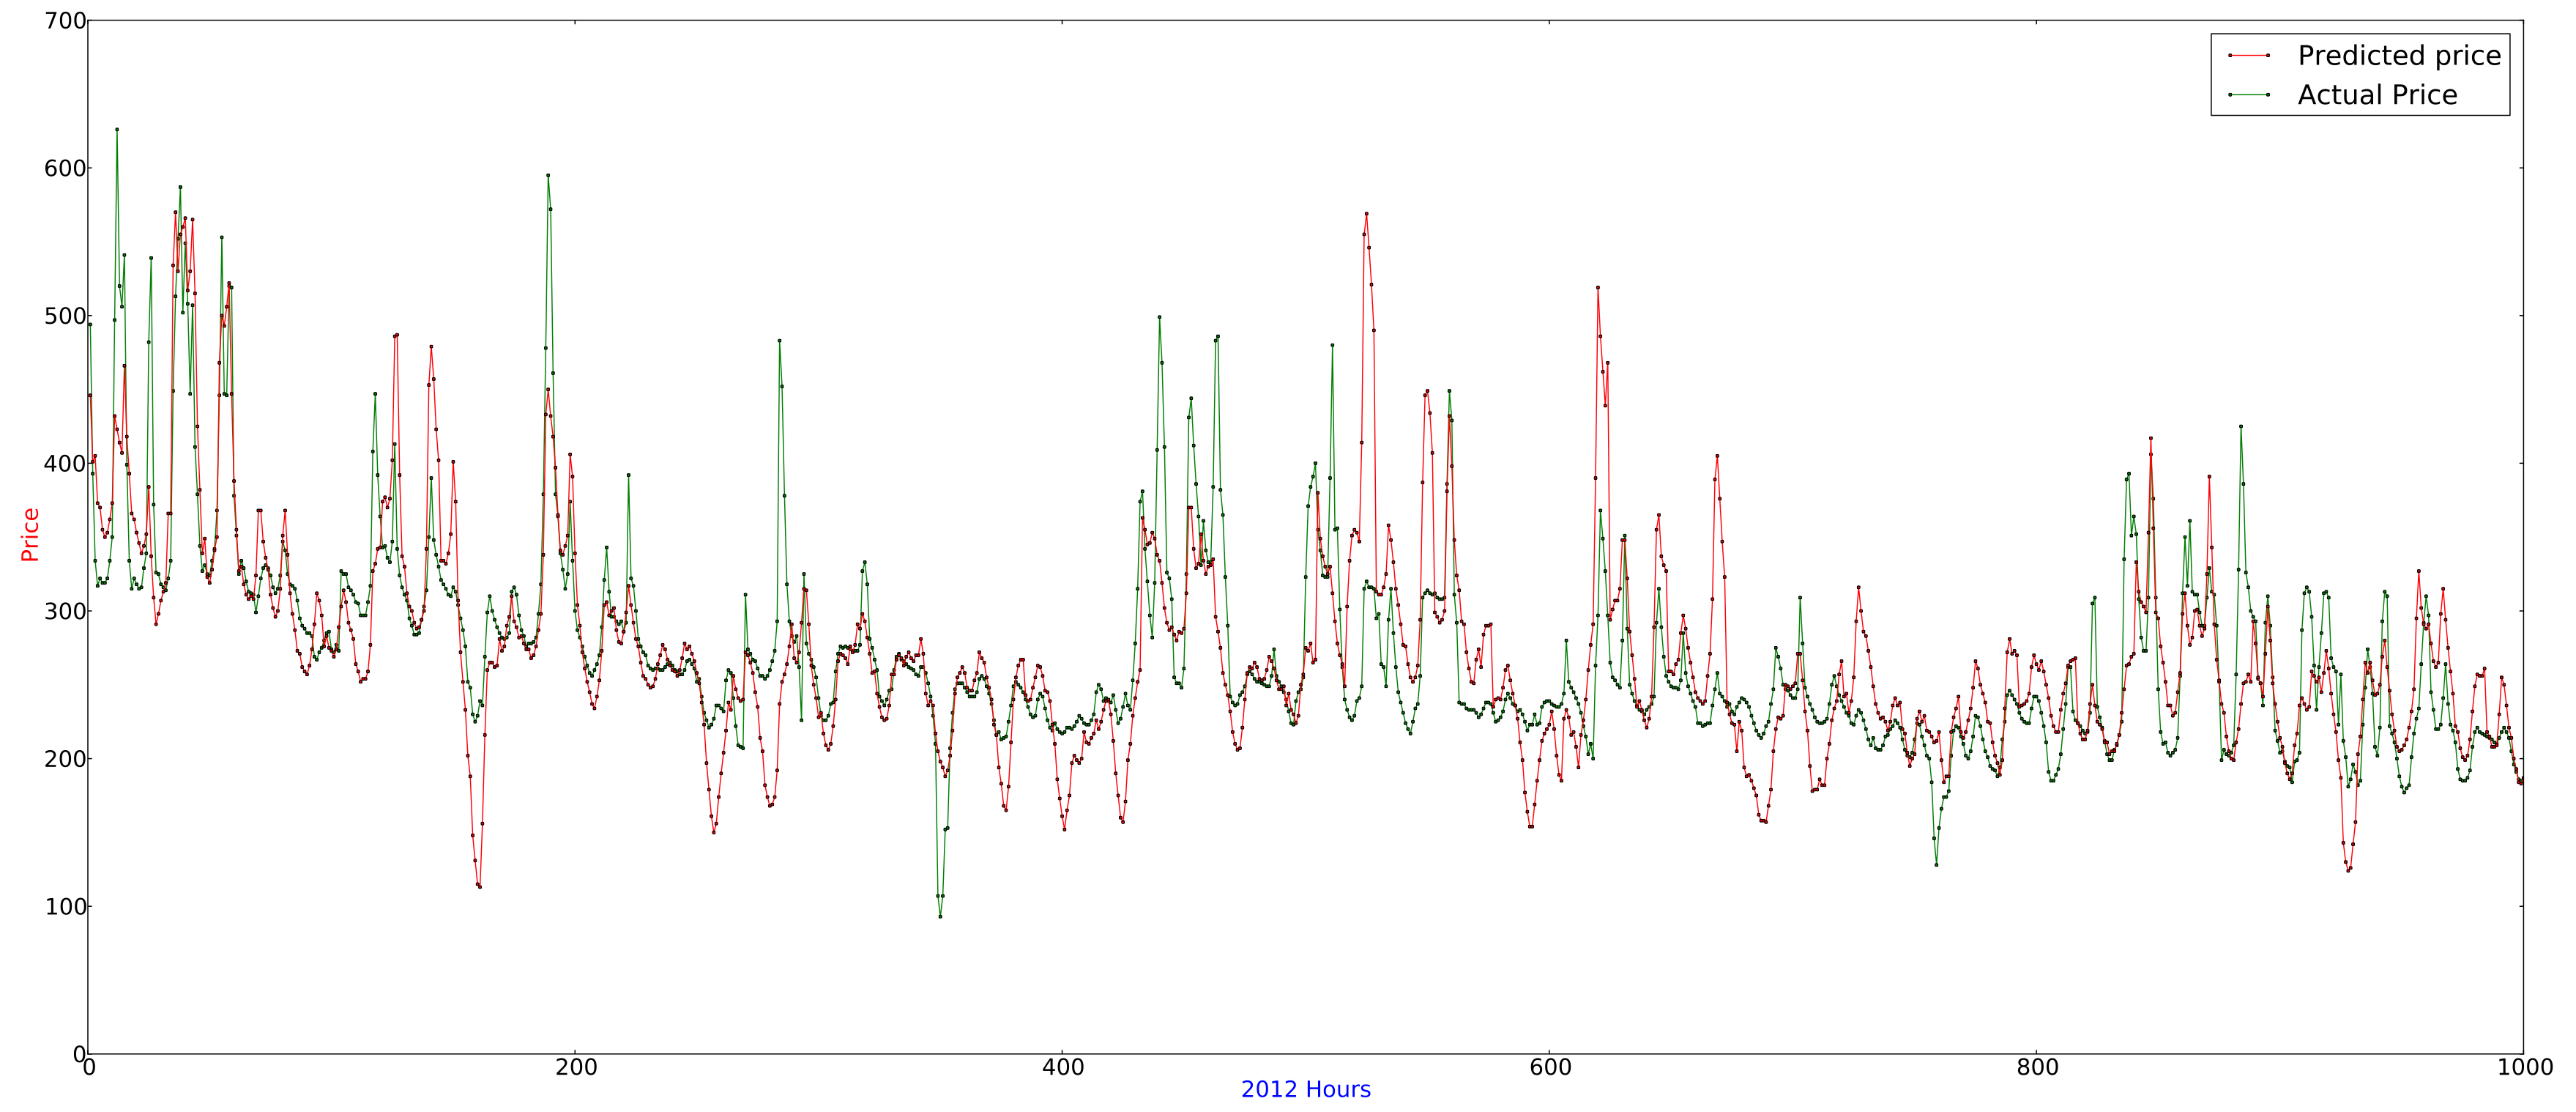
\includegraphics[width=\linewidth]{billeder/PriceGraphs/Experiment2.png}
\caption{First 1000 hours of the best prediction in experiment two}
\label{fig:fullPageExperiment2}
\end{sidewaysfigure}

\subsection{Experiment Three}
The 1000 hour graph Figure is shown in \ref{fig:fullPageExperiment3} for the best prediction from Experiment Three. The full graph can be seen in the digitalized version. In the directory "PriceGraphExperiment3".

\begin{sidewaysfigure}[h]
\centering
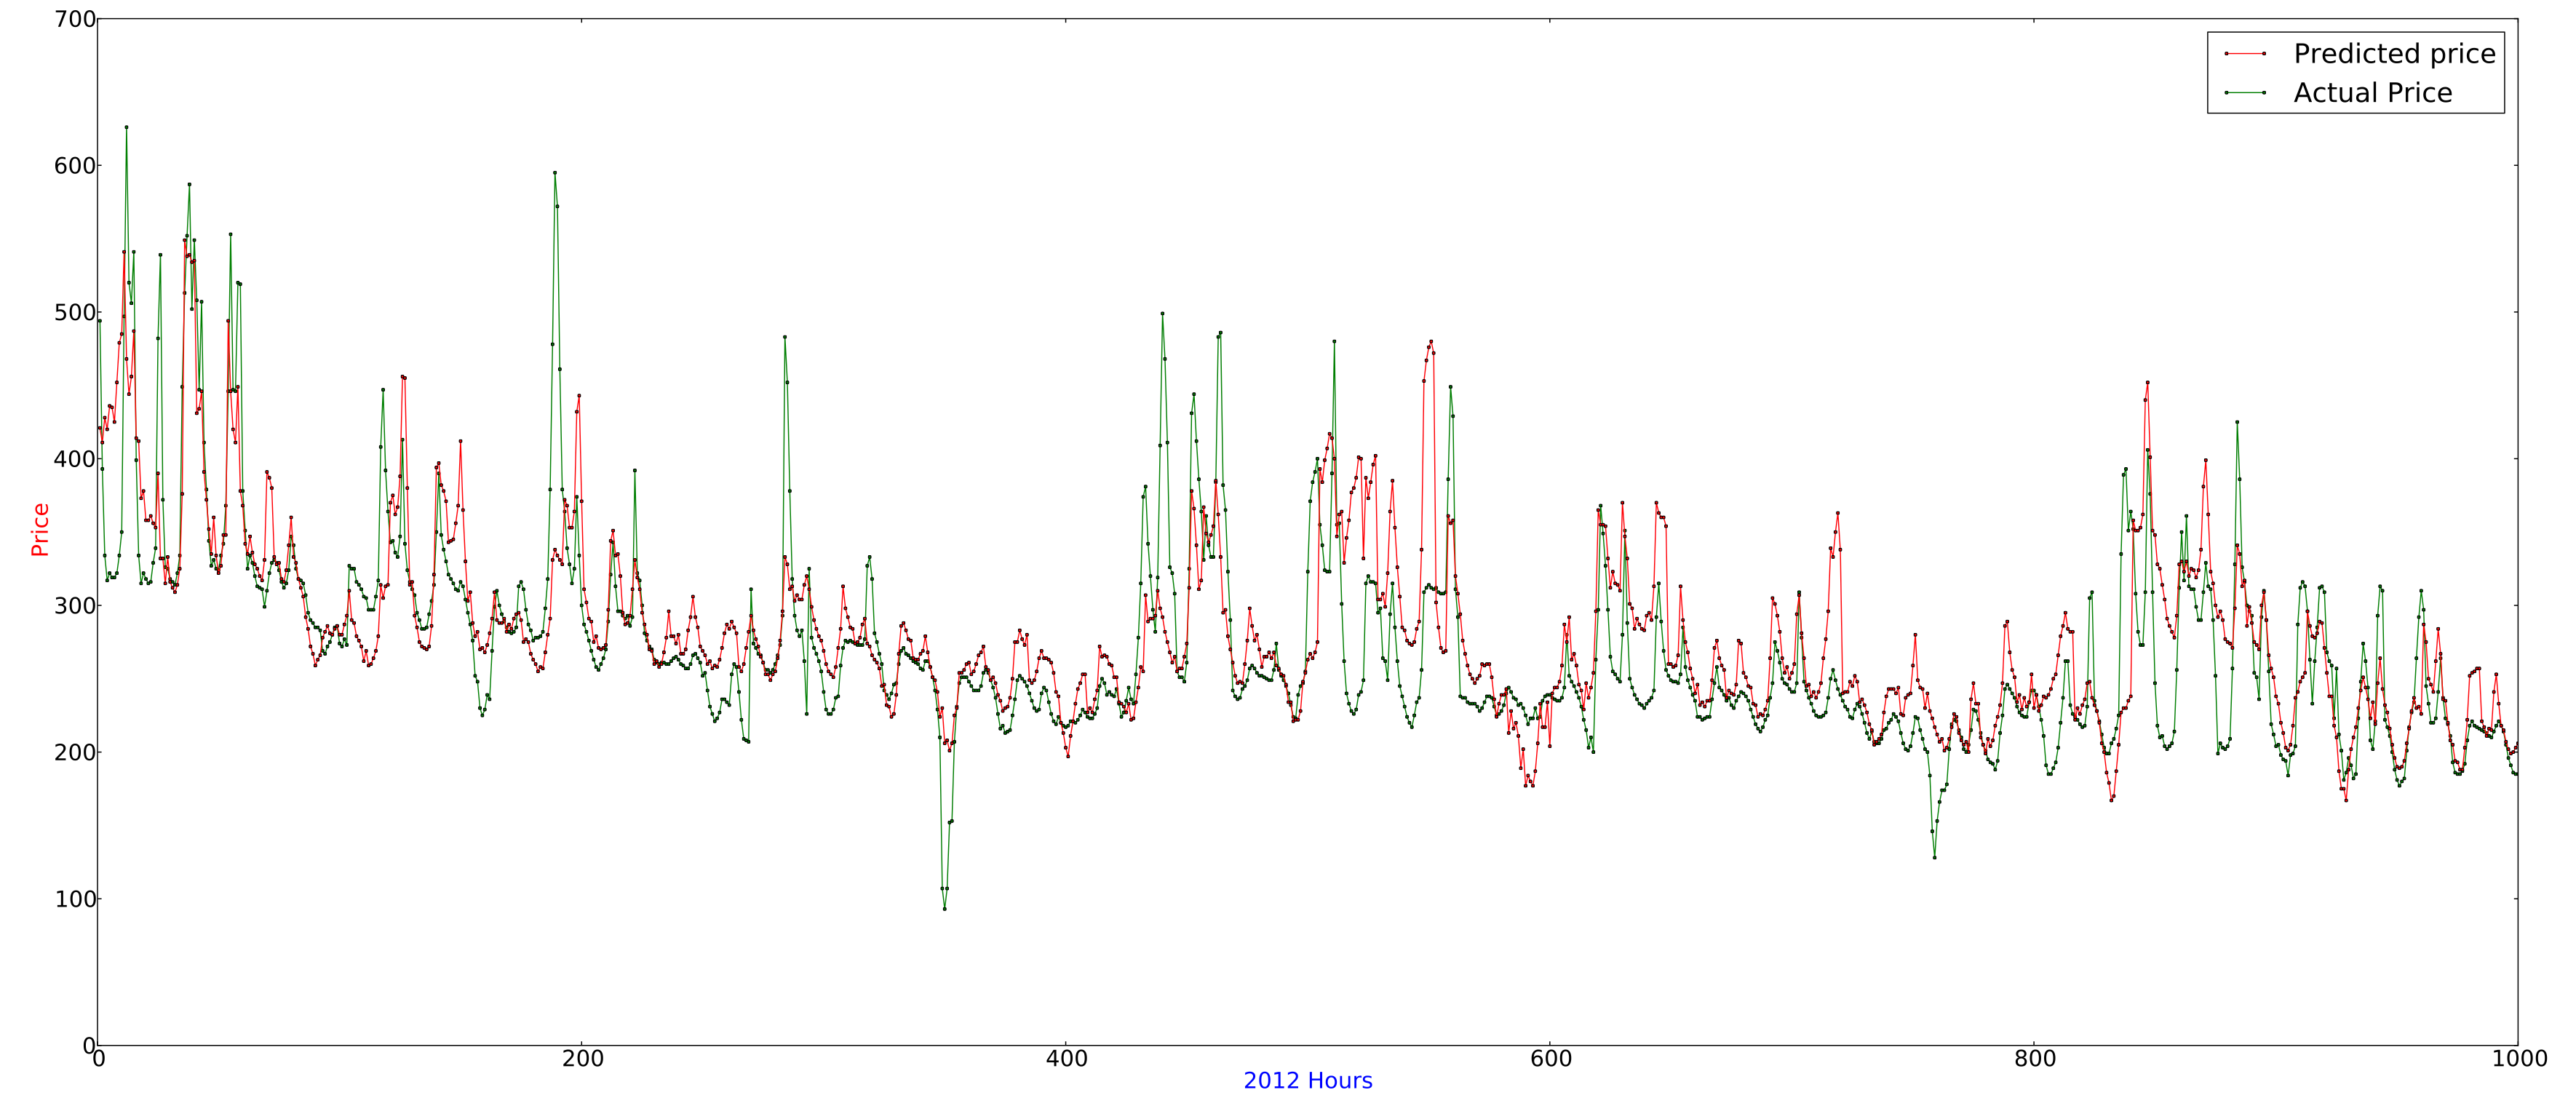
\includegraphics[width=\linewidth]{billeder/PriceGraphs/Experiment3.png}
\caption{First 1000 hours of the best prediction in experiment 3}
\label{fig:fullPageExperiment3}
\end{sidewaysfigure}

\footnotesize
\begin{longtable}{|c|c|c|c|c|c|c|}
\caption{Own set vs Unseen set, Including MAPE}\\
\hline
\textbf{\#} & \textbf{Stack size} & \textbf{Smoothing factor} & \textbf{\% CD} & \textbf{MAPE} & \textbf{MAE} & \textbf{\% ranking} \\
\hline
\endfirsthead
\multicolumn{7}{c}%
{\tablename\ \thetable\ -- \textit{Continued from previous page}} \\
\hline
\textbf{\#} & \textbf{Stack size} & \textbf{Smoothing factor} & \textbf{\% CD} & \textbf{MAPE} & \textbf{MAE} & \textbf{\% ranking} \\
\hline
\endhead
\hline \multicolumn{7}{r}{\textit{Continued on next page}} \\
\endfoot
\hline
\endlastfoot
1  & 16 & 0,9 &  67,1\% & 17,56\% & 45,96 & - \\ \hline
2  & 12 & 0,1 &  66,7\% & 17,63\% & 46,13 & 0,38\% \\ \hline
3  & 20 & 0,9 &  66,9\% & 17,76\% & 46,47 & 1,11\% \\ \hline
4  & 8 & 0,9 &  67,1\% & 17,79\% & 46,55 & 1,28\% \\ \hline
5  & 20 & 0,5 &  66,7\% & 17,79\% & 46,56 & 1,31\% \\ \hline
6  & 24 & 0,4 &  67,3\% & 17,80\% & 46,58 & 1,36\% \\ \hline
7  & 20 & 0,7 &  66,4\% & 17,80\% & 46,59 & 1,37\% \\ \hline
8  & 12 & 0,9 &  67,9\% & 17,81\% & 46,61 & 1,41\% \\ \hline
9  & 24 & 0,8 &  67,8\% & 17,88\% & 46,78 & 1,79\% \\ \hline
10 & 24 & 0,5 &  67,1\% & 17,91\% & 46,88 & 2,0\% \\ \hline
11 & 20 & 0,4 &  66,2\% & 17,97\% & 47,03 & 2,33\% \\ \hline
12 & 24 & 0,2 &  67,5\% & 17,97\% & 47,04 & 2,34\% \\ \hline
13 & 12 & 0,3 &  67,6\% & 17,99\% & 47,07 & 2,43\% \\ \hline
14 & 16 & 0,8 &  67,8\% & 18,02\% & 47,17 & 2,63\% \\ \hline
15 & 6 & 0,9 &  67,5\% & 18,10\% & 47,36 & 3,04\% \\ \hline
16 & 16 & 0,6 &  67,3\% & 18,20\% & 47,64 & 3,66\% \\ \hline
17 & 6 & 0,7 &  67,8\% & 18,22\% & 47,69 & 3,77\% \\ \hline
18 & 20 & 0,1 &  67,2\% & 18,25\% & 47,76 & 3,92\% \\ \hline
19 & 24 & 0,3 &  68,0\% & 18,29\% & 47,86 & 4,13\% \\ \hline
20 & 4 & 0,9 &  67,7\% & 18,29\% & 47,86 & 4,14\% \\ \hline
21 & 24 & 0,6 &  67,5\% & 18,29\% & 47,87 & 4,15\% \\ \hline
22 & 4 & 0,5 &  68,9\% & 18,30\% & 47,88 & 4,19\% \\ \hline
23 & 8 & 0,2 &  67,3\% & 18,32\% & 47,94 & 4,3\% \\ \hline
24 & 20 & 0,6 &  67,4\% & 18,32\% & 47,96 & 4,35\% \\ \hline
25 & 6 & 0,2 &  66,9\% & 18,35\% & 48,03 & 4,5\% \\ \hline
26 & 8 & 0,7 &  66,4\% & 18,37\% & 48,08 & 4,61\% \\ \hline
27 & 20 & 0,8 &  66,9\% & 18,39\% & 48,14 & 4,74\% \\ \hline
28 & 20 & 0,2 &  66,6\% & 18,40\% & 48,15 & 4,78\% \\ \hline
29 & 12 & 0,5 &  67,9\% & 18,43\% & 48,22 & 4,92\% \\ \hline
30 & 16 & 0,3 &  66,7\% & 18,43\% & 48,23 & 4,94\% \\ \hline
31 & 16 & 0,7 &  67,1\% & 18,45\% & 48,28 & 5,05\% \\ \hline
32 & 12 & 0,8 &  66,7\% & 18,46\% & 48,32 & 5,13\% \\ \hline
33 & 16 & 0,5 &  66,7\% & 18,50\% & 48,40 & 5,32\% \\ \hline
34 & 24 & 0,7 &  67,0\% & 18,52\% & 48,47 & 5,46\% \\ \hline
35 & 8 & 0,3 &  67,2\% & 18,58\% & 48,63 & 5,81\% \\ \hline
36 & 20 & 0,3 &  67,1\% & 18,58\% & 48,63 & 5,82\% \\ \hline
37 & 8 & 0,6 &  66,4\% & 18,61\% & 48,70 & 5,97\% \\ \hline
38 & 16 & 0,4 &  67,7\% & 18,61\% & 48,71 & 5,98\% \\ \hline
39 & 8 & 0,4 &  67,7\% & 18,63\% & 48,76 & 6,1\% \\ \hline
40 & 6 & 0,1 &  66,3\% & 18,69\% & 48,92 & 6,44\% \\ \hline
41 & 8 & 0,1 &  67,5\% & 18,70\% & 48,94 & 6,48\% \\ \hline
42 & 16 & 0,2 &  68,2\% & 18,75\% & 49,07 & 6,77\% \\ \hline
43 & 16 & 0,1 &  68,0\% & 18,78\% & 49,14 & 6,92\% \\ \hline
44 & 8 & 0,8 &  67,4\% & 18,86\% & 49,35 & 7,37\% \\ \hline
45 & 12 & 0,7 &  67,2\% & 18,89\% & 49,43 & 7,55\% \\ \hline
46 & 6 & 0,5 &  66,8\% & 18,89\% & 49,44 & 7,57\% \\ \hline
47 & 12 & 0,6 &  67,1\% & 18,93\% & 49,54 & 7,79\% \\ \hline
48 & 6 & 0,4 &  67,0\% & 18,96\% & 49,63 & 7,99\% \\ \hline
49 & 24 & 0,1 &  66,9\% & 18,98\% & 49,68 & 8,1\% \\ \hline
50 & 4 & 0,2 &  68,5\% & 19,01\% & 49,74 & 8,22\% \\ \hline
51 & 4 & 0,3 &  67,8\% & 19,05\% & 49,85 & 8,47\% \\ \hline
52 & 6 & 0,6 &  66,4\% & 19,06\% & 49,89 & 8,55\% \\ \hline
53 & 4 & 0,7 &  67,6\% & 19,06\% & 49,89 & 8,55\% \\ \hline
54 & 24 & 0,9 &  66,8\% & 19,07\% & 49,90 & 8,57\% \\ \hline
55 & 4 & 0,8 &  67,5\% & 19,14\% & 50,08 & 8,97\% \\ \hline
56 & 12 & 0,4 &  67,2\% & 19,17\% & 50,18 & 9,18\% \\ \hline
57 & 6 & 0,8 &  67,2\% & 19,22\% & 50,29 & 9,42\% \\ \hline
58 & 8 & 0,5 &  67,5\% & 19,28\% & 50,44 & 9,76\% \\ \hline
59 & 4 & 0,1 &  67,5\% & 19,31\% & 50,52 & 9,94\% \\ \hline
60 & 12 & 0,2 &  67,2\% & 19,37\% & 50,70 & 10,33\% \\ \hline
61 & 4 & 0,4 &  67,6\% & 19,38\% & 50,71 & 10,34\% \\ \hline
62 & 4 & 0,6 &  67,1\% & 19,43\% & 50,84 & 10,62\% \\ \hline
63 & 6 & 0,3 &  67,3\% & 19,63\% & 51,38 & 11,8\% \\ \hline
	\end{longtable}
\normalsize


\subsection{Experiment Four}
The 1000 hour graph Figure is shown in \ref{fig:fullPageExperiment4} for the best prediction from Experiment Four. The full graph can be seen in the digitalized version. In the directory "PriceGraphExperiment4".

\begin{sidewaysfigure}[h]
\centering
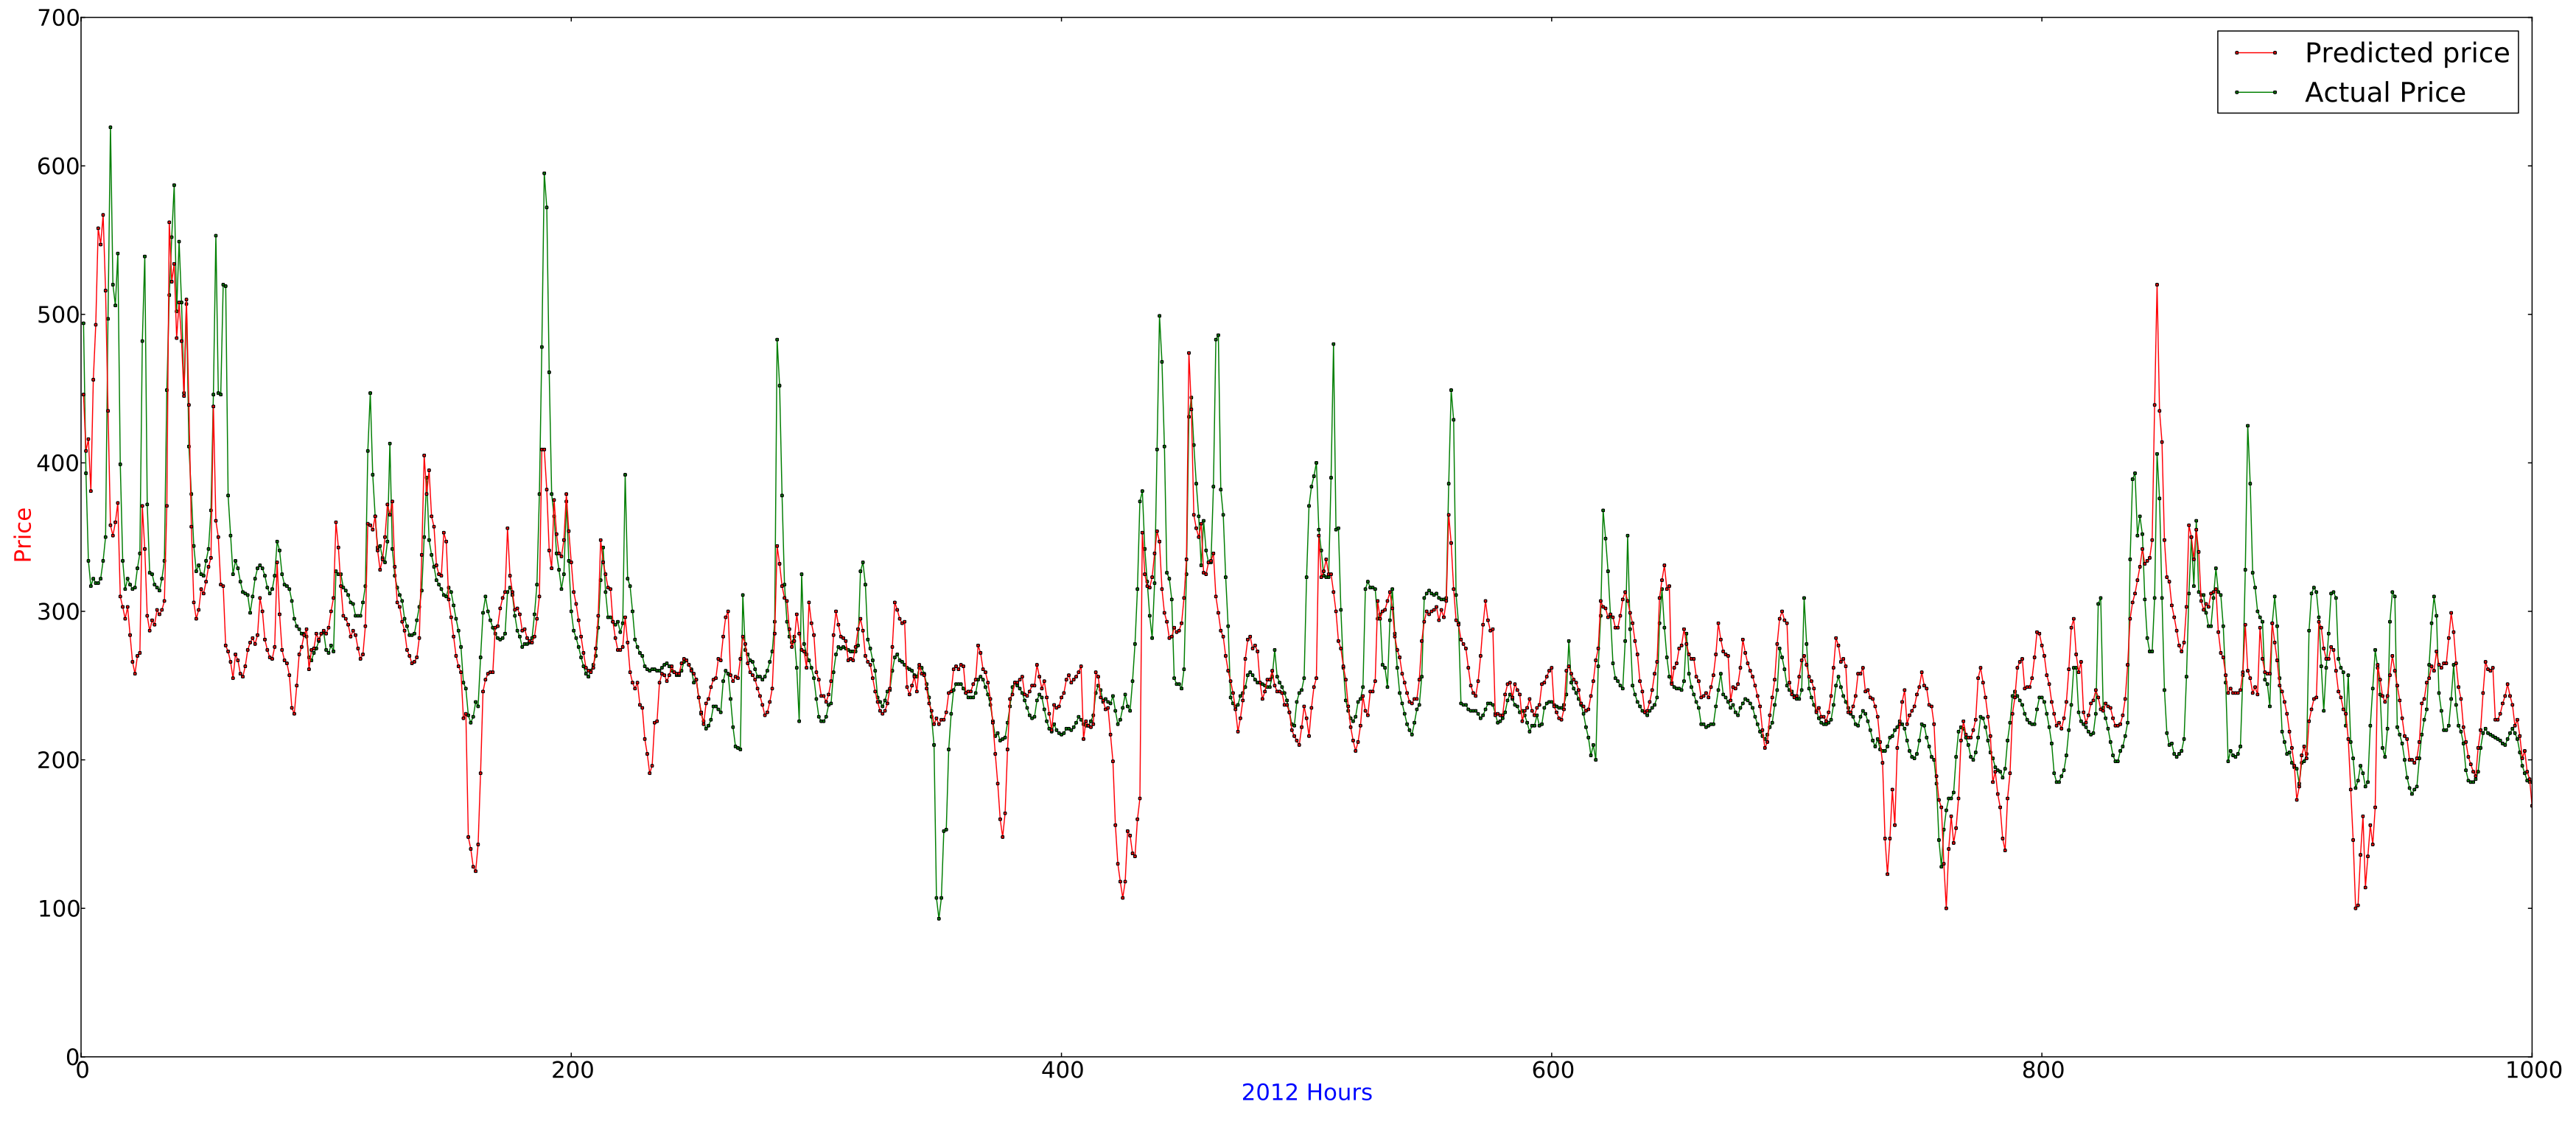
\includegraphics[width=\linewidth]{billeder/PriceGraphs/Experiment4.png}
\caption{First 1000 hours of the best prediction in experiment four}
\label{fig:fullPageExperiment4}
\end{sidewaysfigure}


\subsection{Experiment Five}
The 1000 hour graph Figure is shown in \ref{fig:fullPageExperiment5} for the best prediction from Experiment Five. The full graph can be seen in the digitalized version. In the directory "PriceGraphExperiment5".

\begin{sidewaysfigure}[h]
\centering
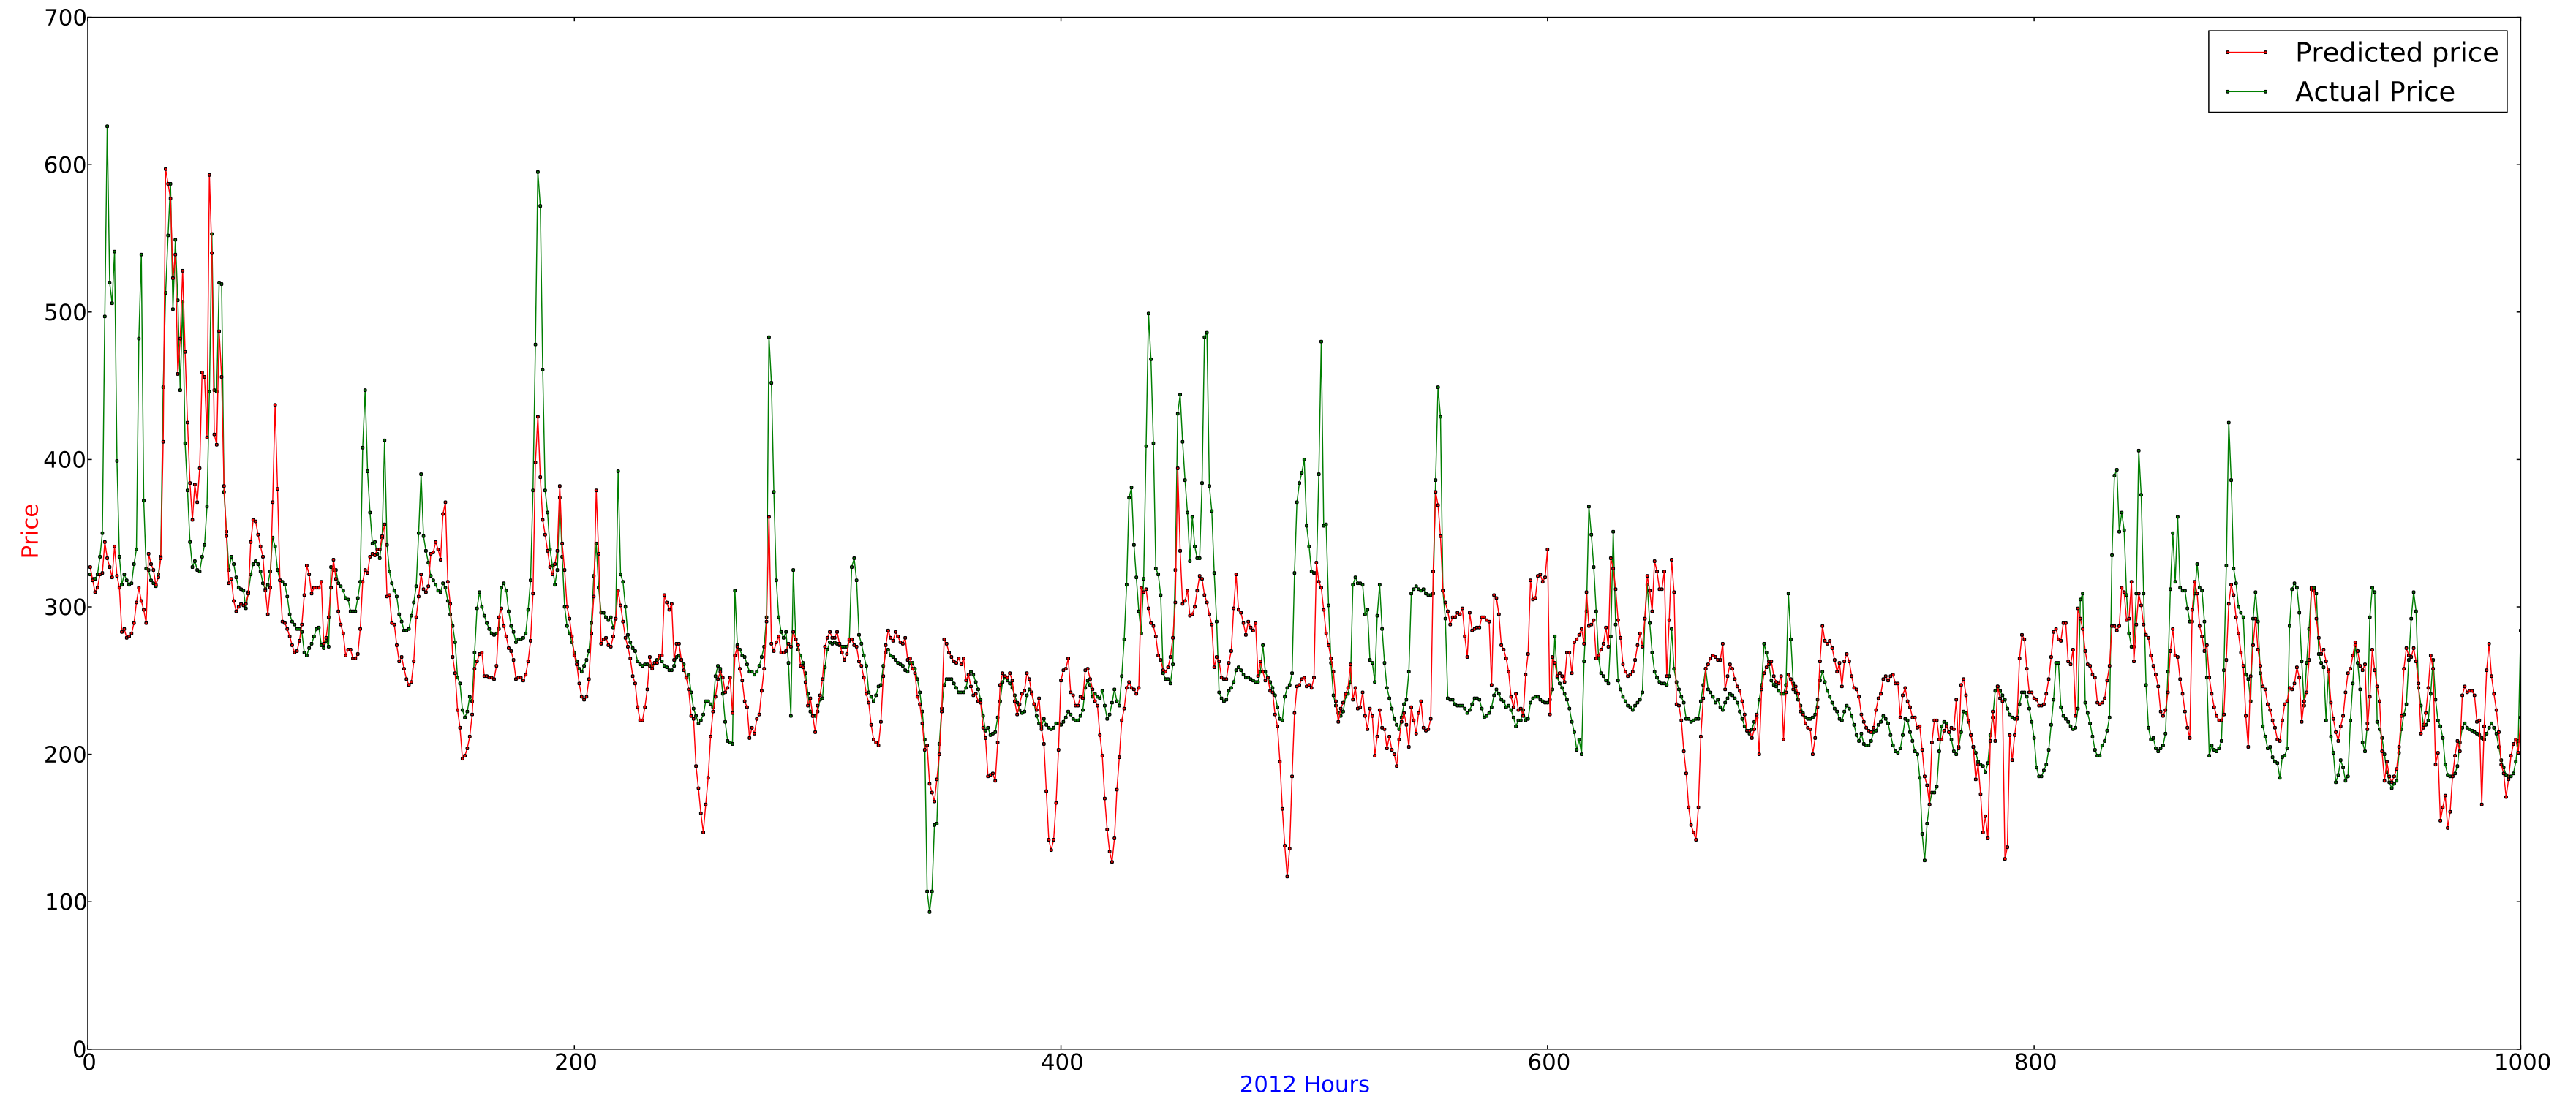
\includegraphics[width=\linewidth]{billeder/PriceGraphs/Experiment5.png}
\caption{First 1000 hours of the best prediction in experiment five}
\label{fig:fullPageExperiment5}
\end{sidewaysfigure}